\chapter{Experimentos y resultados}\label{chapter:Results}

En este capítulo se presentan los experimentos realizados para evaluar
el desempeño y los resultados del algoritmo gen\'etico propuesta en este
trabajo para hallar el sistema de ecuaciones diferenciales ordinarias compartimentales que mejor se ajusten a un conjunto de datos.

En la sección~\ref{sec:experimentation1} se describe el marco experimental. La secci\'on~\ref{sec:experimentation2} muestra como se generaron los datos utilizados en los distintos experimentos y cómo se modeló la presencia de ruido en las muestras. En la sección~\ref{sec:experimentation3} se describen los experimentos realizados y sus resultados, y la secci\'on~\ref{sec:experimentation4} se analizan. A continuación se describe el marco experimental.


\section{Consideraciones en la etapa de experimentaci\'on}
\label{sec:experimentation1}
La presente tesis aborda el problema de identificar la estructura de un sistema de ecuaciones diferenciales compartimentales, lineales con respecto a los parámetros, que mejor se ajuste a un conjunto de datos observados. El espacio de búsqueda de posibles modelos compartimentales es combinatoriamente extenso, ya que cada topología de interconexiones entre compartimentos define un sistema de ecuaciones único. Para navegar eficientemente este vasto espacio de soluciones, se propone una metodología basada en \textbf{algoritmos genéticos}, donde cada posible sistema compartimental es representado mediante una estructura de grafo. La naturaleza estocástica y la carga computacional de los algoritmos genéticos, sumada a la necesidad de evaluar múltiples modelos candidatos en cada generación, justifica el uso de la infraestructura de cómputo de alto rendimiento para la experimentación. Las características del equipo donde se llevaron a cabo los experimentos se detallan a continuación.

\begin{itemize}
    \item \textbf{Servidor:} Dell EMC PowerEdge R640
    \item \textbf{Procesador (CPU):} 96 núcleos de cómputo
    \item \textbf{Memoria RAM:} 512 GB
    \item \textbf{Arquitectura:} 64 bits
    \item \textbf{Sistema Operativo:} Ubuntu 24.04
    \item \textbf{Uso de GPU:} No
\end{itemize}

La implementación algorítmica se desarrolló enteramente en el lenguaje de programación \textbf{Python} (versión 3.12). Se utilizaron bibliotecas especializadas y de amplio uso en la comunidad científica. Entre ellas destacan \textbf{NumPy} \cite{2020NumPy-Array} para operaciones matriciales de alto rendimiento; \textbf{SymPy} \cite{Meurer_SymPy_symbolic_computing_2017} para la construcción y manipulación simbólica de las ecuaciones diferenciales; y \textbf{SciPy} \cite{2020SciPy-NMeth} para la integración numérica de dichas ecuaciones para cada modelo candidato. De manera fundamental, se empleó la biblioteca \textbf{NetworkX} \cite{networkx} para modelar, construir y manipular las topologías de grafos que representan las interconexiones de los sistemas compartimentales. El núcleo de la solución, el \textbf{algoritmo genético} diseñado para evolucionar y encontrar la estructura del grafo óptima, fue una implementación propia desarrollada en el marco de esta investigación, y su código fuente se encuentra disponible en GitHub \cite{comparmentalodesystem2025}.

En la siguiente sección se detalla el procedimiento utilizado para la generación de los datos sintéticos que sirven como base para los experimentos.

\section{Descripci\'on del marco experimental}
\label{sec:experimentation2}

El proceso experimental comienza con la selección de un conjunto de modelos compartimentales conocidos, los cuales son utilizados como base para generar datos sintéticos que emulen escenarios observacionales realistas. Estos modelos representan diferentes estructuras epidemiológicas y varían tanto en complejidad como en número de compartimentos. En total, se consideraron cuatro modelos ampliamente utilizados en la literatura científica: \textbf{SIR}, \textbf{SEIR}, \textbf{SIRD} y \textbf{SEIRV}. Cada uno de ellos modela la evolución de una epidemia bajo distintos supuestos, incluyendo la exposición previa, la vacunación o la presencia de cuarentena y mortalidad.

Para cada modelo se establecieron condiciones iniciales y valores específicos para los parámetros, tomados de ejemplos clásicos o calibrados dentro de rangos razonables. Por ejemplo, para el modelo SIR se utilizó una población inicial distribuida como \( S_0 = 0.99 \), \( I_0 = 0.01 \) y \( R_0 = 0 \), con parámetros de transmisión \( \beta = 0.4 \) y recuperación \( \gamma = 0.1 \). El sistema de ecuaciones diferenciales correspondiente está dado por:

\[
\begin{aligned}
\frac{dS}{dt} &= -\beta SI, \\
\frac{dI}{dt} &= \beta SI - \gamma I, \\
\frac{dR}{dt} &= \gamma I.
\end{aligned}
\]

La integración de estos sistemas se realizó mediante el método \texttt{solve\_ivp} de la biblioteca \texttt{scipy.integrate}, evaluando las soluciones en 150 puntos equiespaciados dentro del intervalo temporal \( t \in [0, 150] \). Este enfoque proporciona una discretización suficiente para capturar la dinámica de los compartimentos sin generar una sobrecarga computacional innecesaria.

La Figura~\ref{fig:sir_sin_ruido} muestra la evolución simulada de los compartimentos del modelo SIR sin presencia de ruido, donde se observa claramente la transición típica entre susceptibles, infectados y recuperados.

\begin{figure}[htbp]
    \centering
    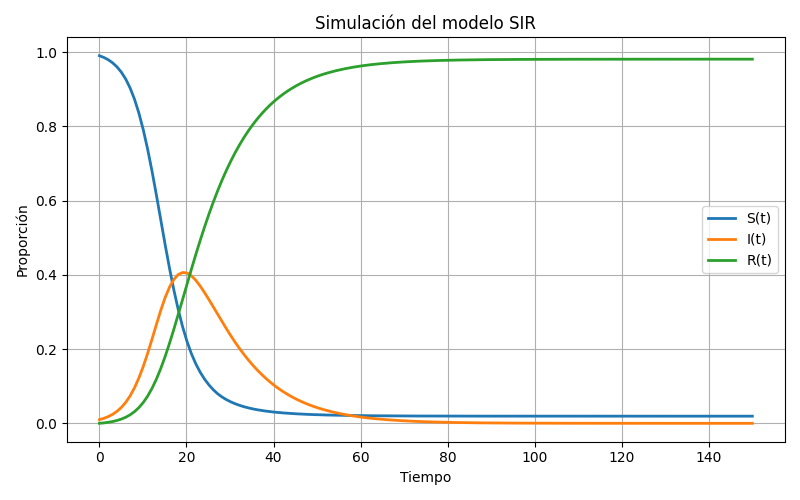
\includegraphics[width=0.7\textwidth]{Graphics/SIR_points.png}
    \caption{Simulación del modelo SIR sin ruido.}
    \label{fig:sir_sin_ruido}
\end{figure}

Una vez obtenidas las trayectorias libres de ruido para cada compartimento, se procedió a simular un entorno más cercano a situaciones reales introduciendo ruido aleatorio. Específicamente, se añadió ruido aditivo con distribución normal a cada punto de los datos. El nivel de ruido se controló mediante un parámetro denominado \texttt{max\_noise}, que representa la desviación estándar del ruido aplicado. Se consideraron tres niveles: 5\%, 15\,\% y 30\,\%, lo cual permite evaluar la robustez de los métodos posteriores frente a diferentes grados de perturbación. La expresión utilizada para generar los datos ruidosos fue:

\[
y_i^{\text{noise}} = y_i + \varepsilon, \quad \varepsilon \sim \mathcal{N}(0, \sigma),
\]

donde \( \sigma = \texttt{max\_noise} \). Cabe señalar que este tipo de ruido es aditivo y no proporcional al valor del compartimento, lo cual evita que variables pequeñas sean afectadas de manera desproporcionada.

La Figura~\ref{fig:sir_con_ruido} presenta una visualización de los datos del modelo SIR con un nivel de ruido del 30\,\%, donde se puede observar la dispersión introducida sobre los puntos originales, simulando así condiciones más próximas a mediciones empíricas.

\begin{figure}[htbp]
    \centering
    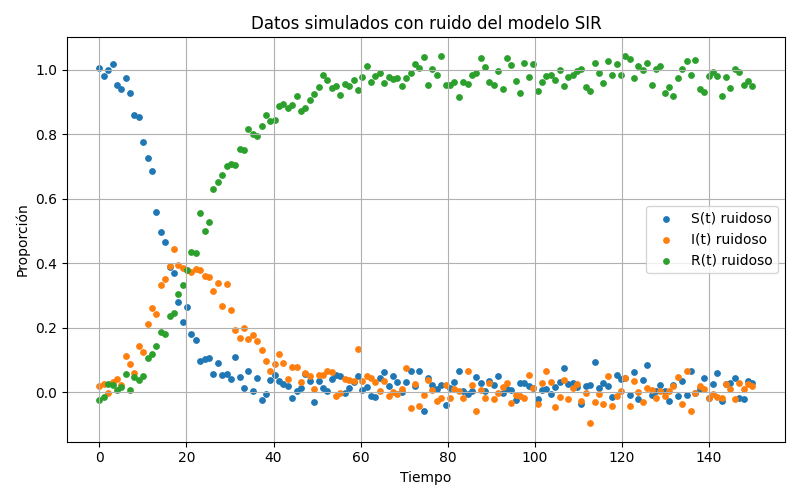
\includegraphics[width=0.7\textwidth]{Graphics/SIR_point_noise.png}
    \caption{Datos simulados del modelo SIR con ruido aditivo de nivel 3\,\%.}
    \label{fig:sir_con_ruido}
\end{figure}

Los conjuntos de datos generados se almacenaron como archivos \texttt{.csv}, con columnas correspondientes al tiempo y a cada compartimento del modelo. La nomenclatura de los archivos incluye el nombre del modelo y el nivel de ruido aplicado, facilitando su posterior identificación y análisis. En total, se produjeron 18 archivos (6 modelos combinados con 3 niveles de ruido), los cuales se emplean como entrada para las siguientes etapas del proceso, incluyendo ajuste de modelos, regresión simbólica y evaluación mediante algoritmos evolutivos.

Esta metodología de generación de datos proporciona un entorno controlado y reproducible para realizar pruebas experimentales, permitiendo estudiar de manera sistemática el desempeño de diferentes estrategias de modelado bajo condiciones con y sin ruido.

En la siguiente sección se presentan los resultados obtenidos en los experimentos realizados para los modelos \textbf{SIR}, \textbf{SEIR}, \textbf{SIRD}, \textbf{SEIRV} y \textbf{SIQRD}, con diferentes valores de ruido en los datos.

\section{Experimentos realizados}
\label{sec:experimentation3}

El experimento tiene como objetivo evaluar la capacidad de un algoritmo genético para inferir estructuras compartimentales, modeladas como sistemas de ecuaciones diferenciales ordinarias (EDOs), a partir de series temporales generadas por modelos epidémicos. Para ello, se desarrolló un marco computacional que transforma automáticamente grafos dirigidos en sistemas compartimentales, ajusta los coeficientes mediante mínimos cuadrados, y evalúa su capacidad predictiva sobre los datos originales.

Cada experimento parte de datos sintéticos generados por un modelo, a los cuales se les añade ruido aleatorio. Este ruido se introduce con diferentes distribuciones y niveles de intensidad, con el objetivo de analizar la robustez del algoritmo ante incertidumbre. Por cada combinación de configuración experimental se ejecutan 30 repeticiones independientes con semillas aleatorias distintas para garantizar diversidad estadística en los resultados.

El proceso de inferencia se realiza mediante un algoritmo genético que evoluciona grafos dirigidos válidos , cada uno representando una posible estructura compartimental. Los parámetros usados incluyen el tamaño de la población, la cantidad de generaciones, y las tasas de mutación y cruzamiento. A lo largo de la evolución, los individuos son evaluados mediante una función de \textit{fitness} basada en el error cuadrático medio (MSE) entre la simulación del modelo inferido y los datos observados. La función incluye penalizaciones adicionales por complejidad estructural, violación de la conservación poblacional, en caso de que se indique, y valores negativos en las simulaciones.

Se evaluaron también diferentes \textit{thresholds} que es el umbral que se define en el Cap\'itulo~\ref{chapter:fitness} en la Secci\'on~\ref{sec:term_sig} para seleccionar los t\'erminos relevantes en las ecuaciones, en este caso se usaron valores de 0.8 y 1.0, para controlar la significancia de los términos en las ecuaciones diferenciales, afectando así la complejidad de los modelos generados.

Por cada ejecución, se registran los siguientes elementos:
\begin{itemize}
    \item El mejor grafo descubierto y sus aristas.
    \item Las ecuaciones diferenciales finales generadas.
    \item El valor de fitness (MSE).
    \item El tiempo total de ejecución.
\end{itemize}

Los resultados obtenidos se presentan en una tabla resumen, donde se comparan las distintas configuraciones experimentales:

\begin{table}[H]
\centering
\caption{Resumen de resultados por configuración experimental}
\begin{tabular}{|c|c|c|c|c|}
\hline
\textbf{Ruido} & \textbf{\textit{Threshold}} & \textbf{Fitness Mín.} & \textbf{MSE} & \textbf{Aristas del grafo} \\
\hline
 &  &  &  &  \\
\hline
\end{tabular}
\label{tab:resultados-experimentales}
\end{table}

\noindent

Los valores de fitness representan el MSE entre la simulación del modelo inferido y los datos originales. Las métricas están promediadas sobre 30 ejecuciones independientes por configuración.

A continuación se presentan los resultados obtenidos para el modelo SIR.

\subsection{Modelo SIR}

El modelo SIR es un marco matemático fundamental que se utiliza para analizar cómo se propaga una enfermedad infecciosa a través de una población \cite{Kermack1927}. El sistema se define como:
\[
\begin{aligned}
\frac{dS}{dt} &= -\beta SI, \\
\frac{dI}{dt} &= \beta SI - \gamma I, \\
\frac{dR}{dt} &= \gamma I.
\end{aligned}
\]
donde S indica la cantidad de personas susceptibles, I la cantidad de personas infectadas y R la cantidad de personas recuperadas. Se utiliza el parámetro $\beta$ para indicar el índice de transmisión y $\gamma$ el índice de recuperación de la enfermedad.

El grafo que representar\'ia este sistema ser\'ia el compuesto por estas aristas: $S \rightarrow I$, $I \rightarrow R$.

Se utilizaron como valores de los parámetros $\beta = 0.4$ y $\gamma = 0.1$ con punto inicial (0.7, 0.3, 0) y se integró en el intervalo $0 \leq t \leq 150$ para obtener los datos que aparecen en la imagen~\ref{fig:sir_sin_ruido}. Del conjunto de puntos se seleccionaron 150 muestras como datos para el algoritmo gen\'etico. 

El algoritmo se ejecuto con los par\'ametros de 30 para la poblaci\'on inicial y 20 el n\'umero de geneaciones.

Los resultados obtenidos durante las 30 ejecuciones del algoritmo genético sobre los datos generados por el modelo SIR se resumen en la Tabla~\ref{tab:resumen-sir}. En ella se muestran las configuraciones correspondientes a diferentes niveles de ruido y valores de \textit{threshold} (0.8 y 1.0) utilizados para filtrar los términos significativos en las ecuaciones diferenciales. Para cada combinación se reporta el mejor valor de \textit{fitness}, el error cuadrático medio (MSE) en validación y la estructura del grafo inferido.

\begin{table}[H]
\centering
\caption{Resumen de las mejores soluciones para el modelo SIR bajo distintas configuraciones}
\label{tab:resumen-sir}
\begin{tabular}{|c|c|c|c|c|}
\hline
\textbf{Ruido} & \textbf{\textit{Threshold}} & \textbf{Fitness} & \textbf{MSE Validación} & \textbf{Aristas del Grafo} \\
\hline
5\% & 0.8 & 0.00008170 & 0.00007718 & 0 $\rightarrow$ 1, 1 $\rightarrow$ 2 \\
5\% & 1.0 & 0.00141273 & 0.00133686 & 0 $\rightarrow$ 1, 1 $\rightarrow$ 2 \\
15\% & 0.8 & 0.12484250 & 0.10983983 & 0 $\rightarrow$ 2, 1 $\rightarrow$ 2, 2 $\rightarrow$ 1 \\
15\% & 1.0 & 0.00266643 & 0.00076029 & 0 $\rightarrow$ 1, 1 $\rightarrow$ 2 \\
30\% & 0.8 & 0.01876324 & 0.01529640 & 0 $\rightarrow$ 2, 1 $\rightarrow$ 2 \\
30\% & 1.0 & 0.01876324 & 0.01529640 & 0 $\rightarrow$ 2, 1 $\rightarrow$ 2 \\
\hline
\end{tabular}
\end{table}

Las ecuaciones diferenciales asociadas a las mejores soluciones por configuración es la siguiente:
\[
\begin{aligned}
\frac{dS}{dt} &= -0.40199\,S I, \\
\frac{dI}{dt} &= 0.29265\,S I - 0.10328\,I^2 - 0.09670\,I R, \\
\frac{dR}{dt} &= 0.10934\,S I + 0.10328\,I^2 + 0.09670\,I R.
\end{aligned}
\]
En las Figuras~\ref{fig:sir_5p_th08}, \ref{fig:sir_15p_th10} y \ref{fig:sir_30p_th10} se pueden observar las comparaciones entre los datos originales y las simulaciones generadas por los modelos inferidos. Otro sistema de ecuaciones que alcanz\'o buenos resultados en las aproximaci\'on de los datos fue:
\[
\begin{aligned}
\frac{dS}{dt} &= -0.39851\,S I, \\
\frac{dI}{dt} &= 0.23646\,S I - 0.146624\,I R, \\
\frac{dR}{dt} &= 0.16205\,S I + 0.14662\,I R,
\end{aligned}
\]
que representa el conjunto de puntos representados en la Figura~\ref{fig:sir_15p_th10}.

\begin{figure}[H]
\centering
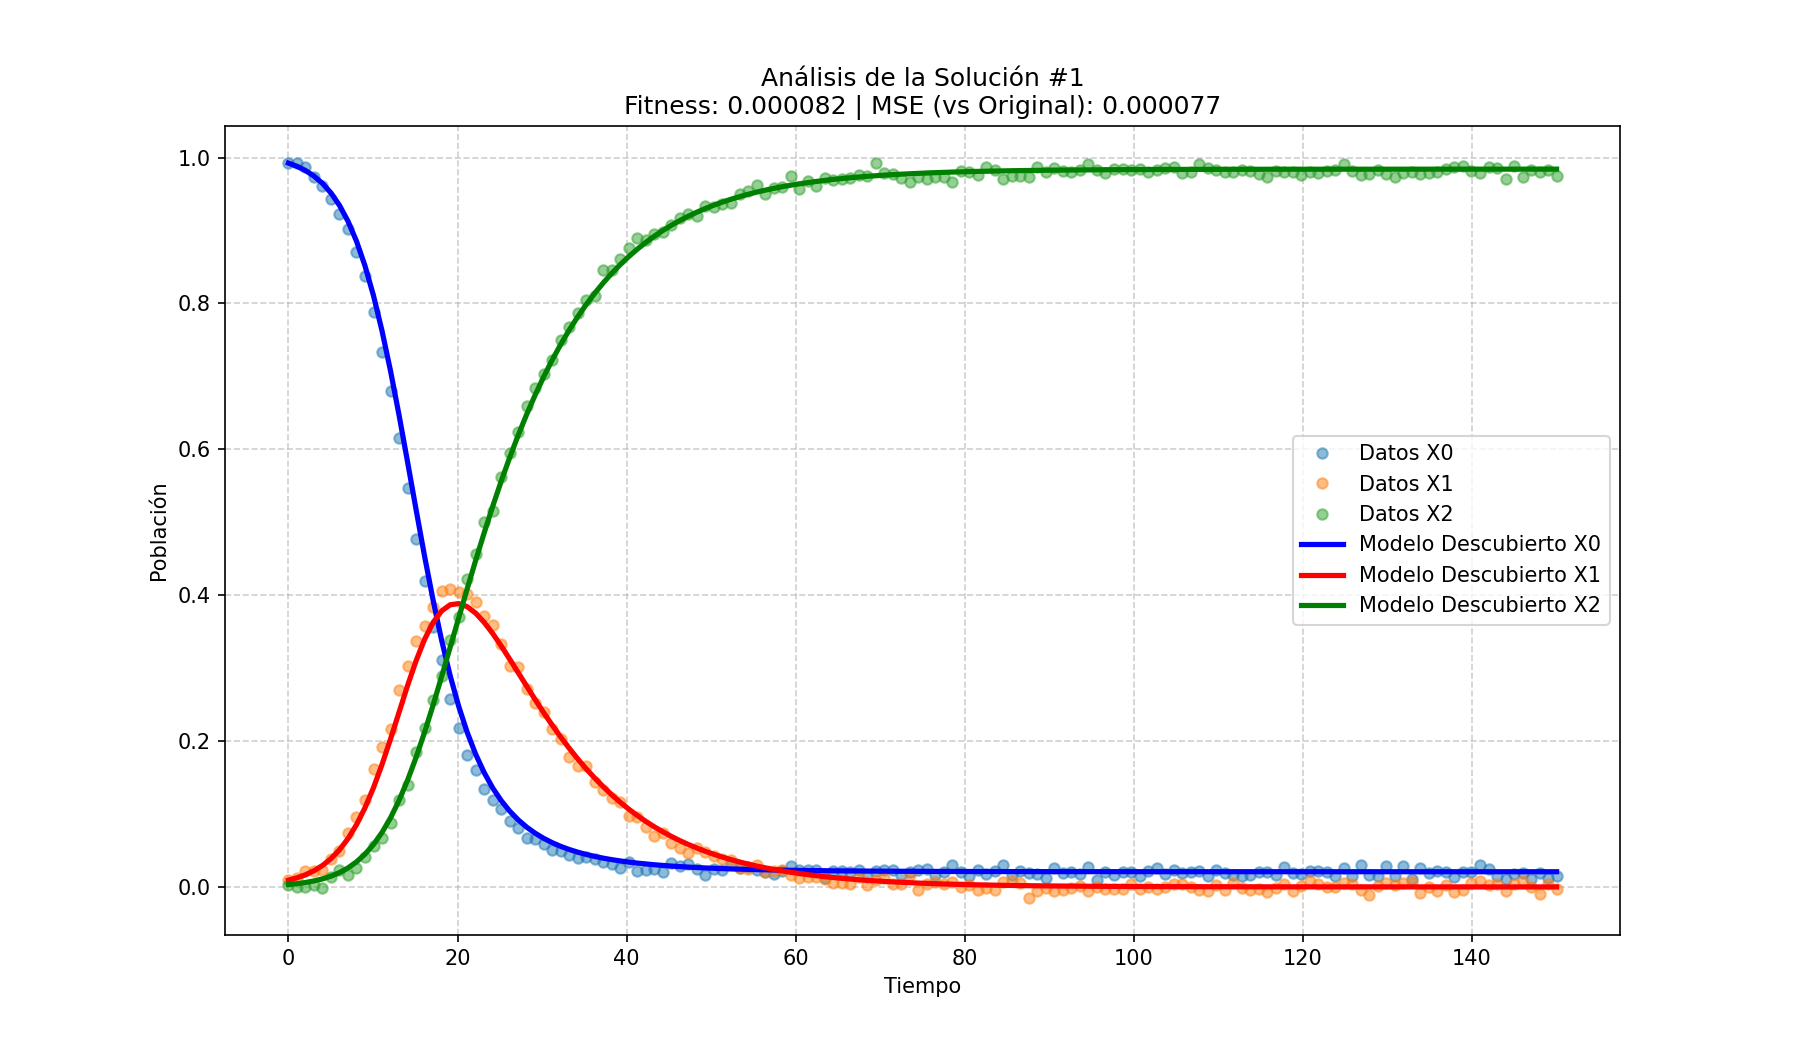
\includegraphics[width=0.7\textwidth]{Graphics/SIR_noise_0p005_0.8_exp10__solution_1.png}
\caption{Simulación del modelo vs datos reales para 5\% de ruido, \textit{threshold} 0.8. $X_0=S , X_1=I, X_2=R$}
\label{fig:sir_5p_th08}
\end{figure}

A pesar del ruido introducido en los datos, los resultados muestran que el sistema inferido logra aproximar adecuadamente el comportamiento dinámico original. En particular, con ruido del 5\,\% y un \textit{threshold} de 0.8, se obtuvo un modelo con error MSE de validación de apenas 7.7e-05 (Figura~\ref{fig:sir_5p_th08}), muy cercano a los datos originales. En contraste, para niveles de ruido más altos como el 30\,\%, aunque las ecuaciones inferidas presentan más términos ajenos al modelo SIR original, los valores de MSE siguen siendo razonables, como se aprecia en la Figura~\ref{fig:sir_30p_th10}.

\begin{figure}[H]
\centering
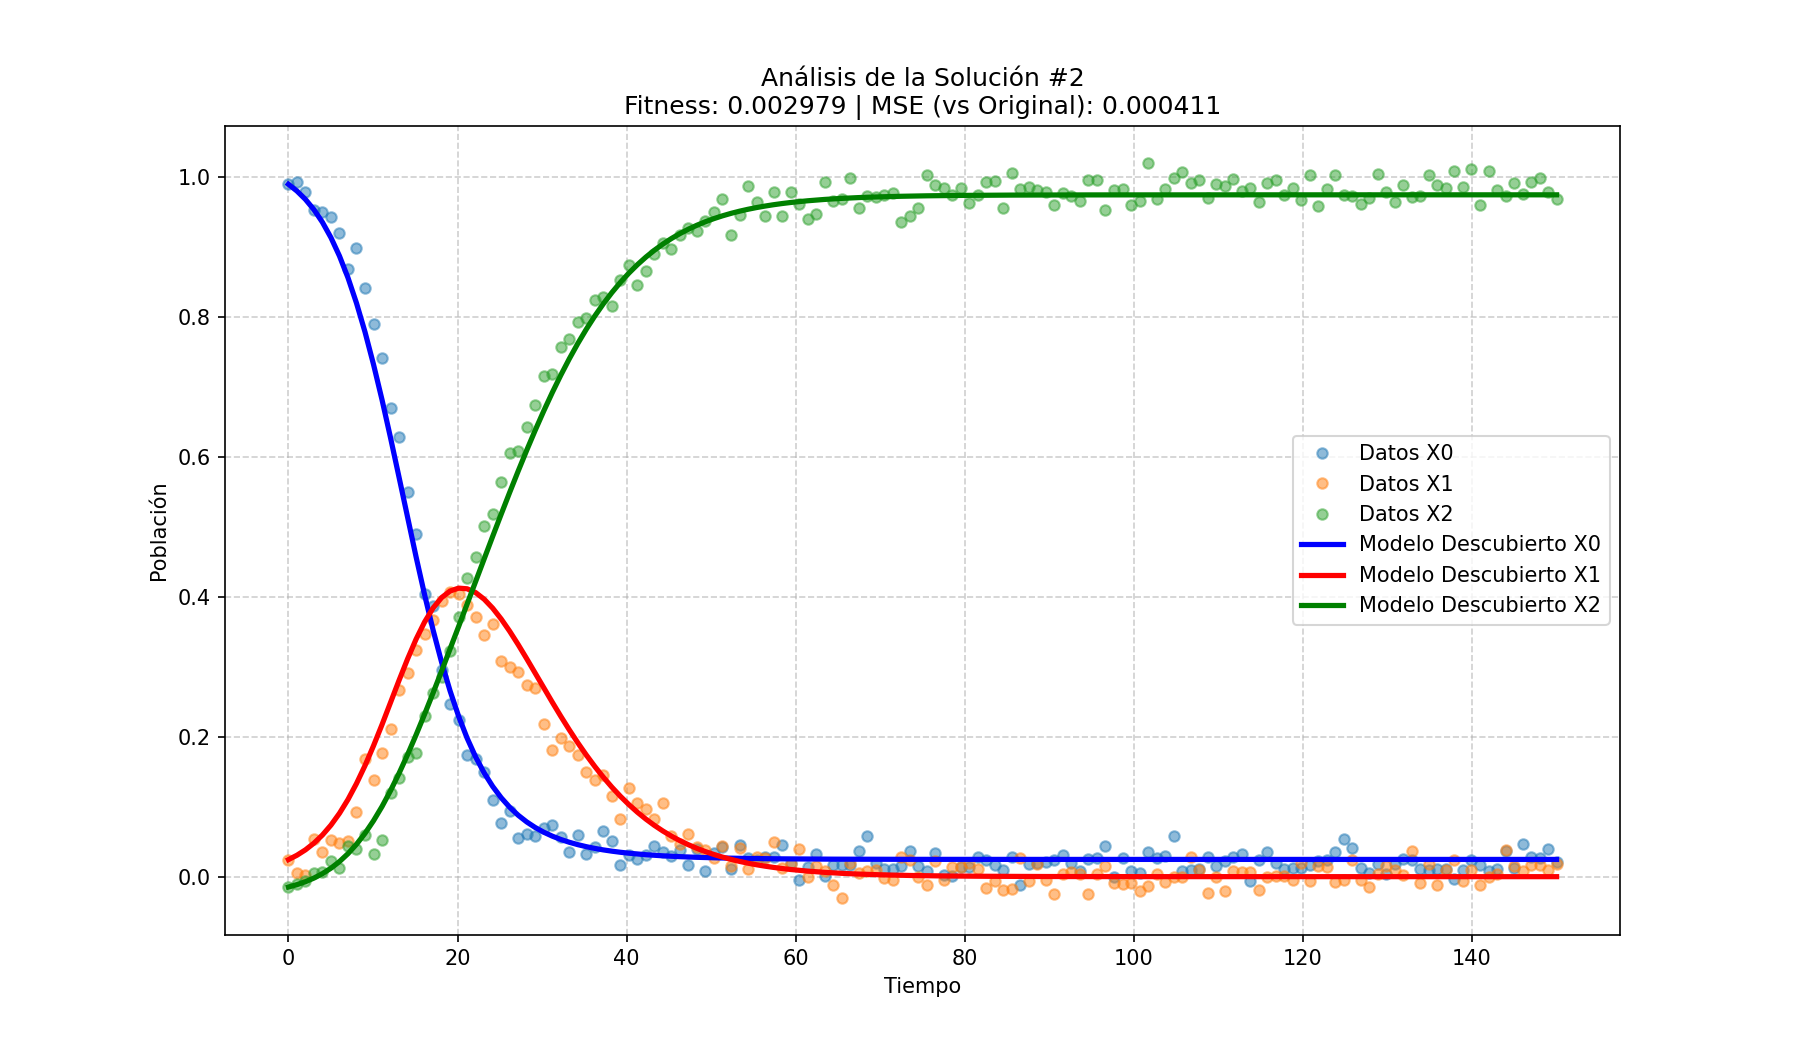
\includegraphics[width=0.7\textwidth]{Graphics/SIR_noise_0p015_1.0_exp10__solution_2.png}
\caption{Simulación del modelo vs datos reales para 15\% de ruido, \textit{threshold} 1.0. $X_0=S , X_1=I, X_2=R$}
\label{fig:sir_15p_th10}
\end{figure}

Es importante destacar que nunca se recuperó exactamente el sistema original que generó los datos. Sin embargo, los modelos inferidos son estructural y dinámicamente consistentes, respetando las restricciones del problema y capturando las tendencias generales del sistema. Esto se refleja en la cercanía entre las trayectorias simuladas y los datos reales en todos los escenarios evaluados. Adem\'as se devuelve correctamente el grafo que representa el modelo SIR.

\begin{figure}[H]
\centering
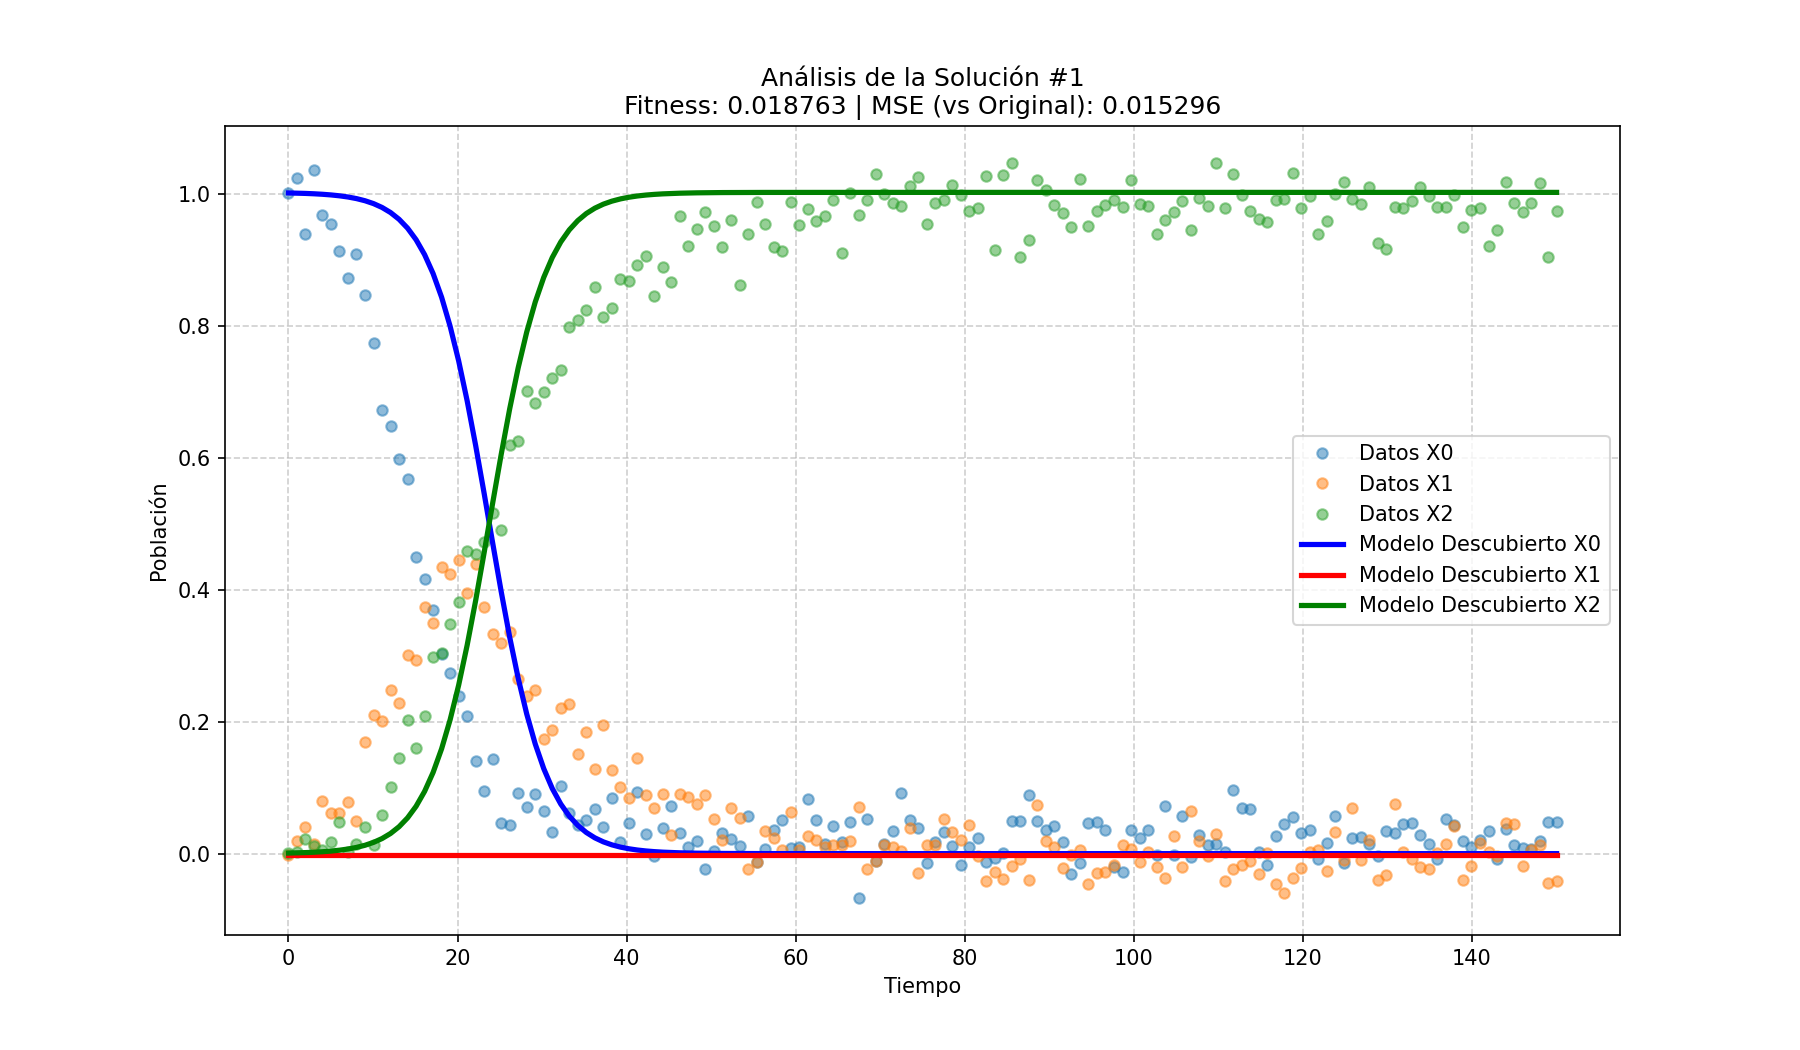
\includegraphics[width=0.7\textwidth]{Graphics/SIR_noise_0p03_1.0_exp18__solution_1.png}
\caption{Simulación del modelo vs datos reales para 30\% de ruido, \textit{threshold} 1.0. $X_0=S , X_1=I, X_2=R$}
\label{fig:sir_30p_th10}
\end{figure}

En condiciones ideales sin ruido y utilizando el sistema original como aproximador de derivadas, se logra una aproximación casi exacta, con valores promedio de fitness del orden de 1e-07.

Resaltar que los tiempos de ejecuci\'on durante cada ejecuci\'on del algoritmo gen\'etico van desde 40 segundos hasta 1 minuto. Estos tiempos son razonables teniendo en cuenta el espacio de b\'usqueda de todos los grafos v\'alidos.

A continuación se presentan los resultados en los experimentos del modelo SEIR.

\subsection{Modelo SEIR}

El modelo SEIR refina al clásico modelo SIR al incorporar un período de latencia de la enfermedad, proporcionando un marco matemático más realista para infecciones donde los individuos no se vuelven infecciosos inmediatamente después del contagio \cite{Hethcote2000}. El sistema se define mediante el siguiente conjunto de ecuaciones diferenciales:
%
\[
\begin{aligned}
    \frac{dS}{dt} &= -\beta SI, \\
    \frac{dE}{dt} &= \beta SI - \alpha E, \\
    \frac{dI}{dt} &= \alpha E - \gamma I, \\
    \frac{dR}{dt} &= \gamma I.
\end{aligned}
\]
%
Donde S representa la proporción de individuos susceptibles, E los expuestos (en período de incubación y no infecciosos), I los infecciosos y R los recuperados. El parámetro $\beta$ controla la tasa de transmisión, $\alpha$ es la tasa a la que los individuos expuestos se vuelven infecciosos, y $\gamma$ es la tasa de recuperación.

El grafo que representa este sistema está compuesto por las siguientes aristas, que ilustran las transiciones posibles entre los compartimentos: $S \rightarrow E \rightarrow I \rightarrow R$.

Se utilizaron como valores de los parámetros $\beta = 0.4$, $\alpha = 0.2$ y $\gamma = 0.1$ con punto inicial (0.9, 0.1, 0, 0) y se integró en el intervalo $0 \leq t \leq 150$ para obtener los datos que aparecen en la imagen~\ref{fig:seir_sin_ruido}. Del conjunto de puntos se seleccionaron 150 muestras como datos para el algoritmo genético.

\begin{figure}[H]
    \centering
    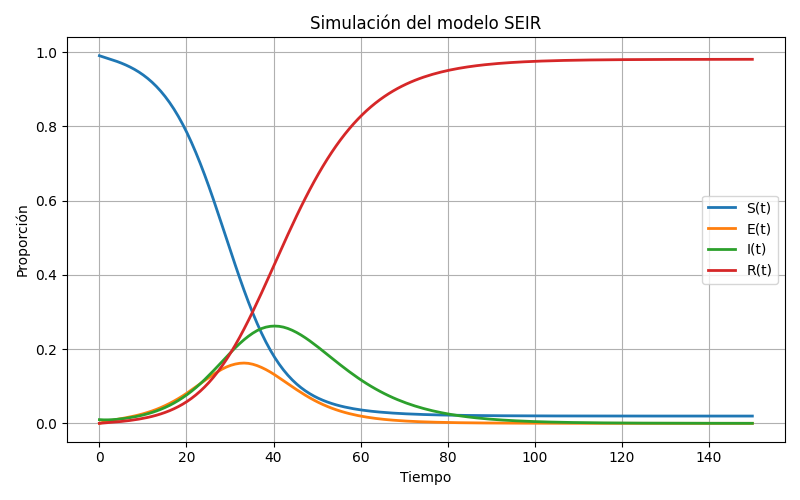
\includegraphics[width=0.7\textwidth]{Graphics/seir_sin_ruido.png}
    \caption{Datos simulados del modelo SEIR}
    \label{fig:seir_sin_ruido}
\end{figure}

El algoritmo se ejecutó con los parámetros de 30 para la población inicial y 20 el número de generaciones.

Los resultados obtenidos durante las 30 ejecuciones del algoritmo genético sobre los datos generados por el modelo SEIR se resumen en la Tabla~\ref{tab:resumen-seir}. En ella se presentan las combinaciones evaluadas según diferentes niveles de ruido en los datos simulados (5\,\%, 15\,\% y 30\,\%) y los valores del parámetro \textit{threshold} (0.8 y 1.0) que determina el criterio de significancia para incluir términos en las ecuaciones diferenciales. Para cada configuración se reporta el mejor valor de \textit{fitness}, el error cuadrático medio (MSE) de validación, y la estructura del grafo inferido que representa las interacciones entre compartimentos.

\begin{table}[H]
\centering
\caption{Resumen de las mejores soluciones para el modelo SEIR bajo distintas configuraciones}
\label{tab:resumen-seir}
\begin{tabular}{|c|c|c|c|c|}
\hline
\textbf{Ruido} & \textbf{\textit{Threshold}} & \textbf{Fitness} & \textbf{MSE Validación} & \textbf{Aristas del Grafo} \\
\hline
5\% & 0.8 & 0.00992 & 0.00586 & 0$\rightarrow$1, 0$\rightarrow$2, 1$\rightarrow$3, 2$\rightarrow$1, 2$\rightarrow$3 \\
5\% & 1.0 & 0.00214 & 0.00123 & 0$\rightarrow$1, 0$\rightarrow$2, 0$\rightarrow$3, 1$\rightarrow$2, 1$\rightarrow$3, 2$\rightarrow$3 \\
15\% & 0.8 & 0.07986 & 0.06807 & 0$\rightarrow$1, 0$\rightarrow$2, 1$\rightarrow$3, 3$\rightarrow$2 \\
15\% & 1.0 & 0.59052 & 0.43875 & 0$\rightarrow$1, 0$\rightarrow$2, 0$\rightarrow$3, 1$\rightarrow$2, 1$\rightarrow$3, 3$\rightarrow$1 \\
30\% & 0.8 & 2.75540 & 0.06372 & 0$\rightarrow$3, 1$\rightarrow$0, 1$\rightarrow$2, 1$\rightarrow$3, 2$\rightarrow$0, 2$\rightarrow$3 \\
30\% & 1.0 & 2.49779 & 0.03656 & 0$\rightarrow$2, 0$\rightarrow$3, 3$\rightarrow$1 \\
\hline
\end{tabular}
\end{table}

\noindent
Para ilustrar los resultados obtenidos, se detallan a continuación las ecuaciones diferenciales correspondientes a algunas de las mejores soluciones halladas. Por ejemplo, en el caso de 5\,\% de ruido y \textit{threshold} de 1.0, la mejor solución obtenida muestra un ajuste muy preciso a los datos originales, con un error cuadrático medio de validación (MSE) de apenas 0.00123. El sistema inferido fue el siguiente:

\[
\begin{aligned}
\frac{dS}{dt} &= -0.40133\,SI - 0.00497\,IR, \\
\frac{dE}{dt} &= 0.19467\,SI - 0.45074\,EI - 0.01597\,IR, \\
\frac{I}{dt} &= 0.12123\,SI + 0.16135\,EI - 0.09800\,IR, \\
\frac{dR}{dt} &= 0.08543\,SI + 0.28939\,EI + 0.11895\,IR.
\end{aligned}
\]

\begin{figure}[H]
\centering
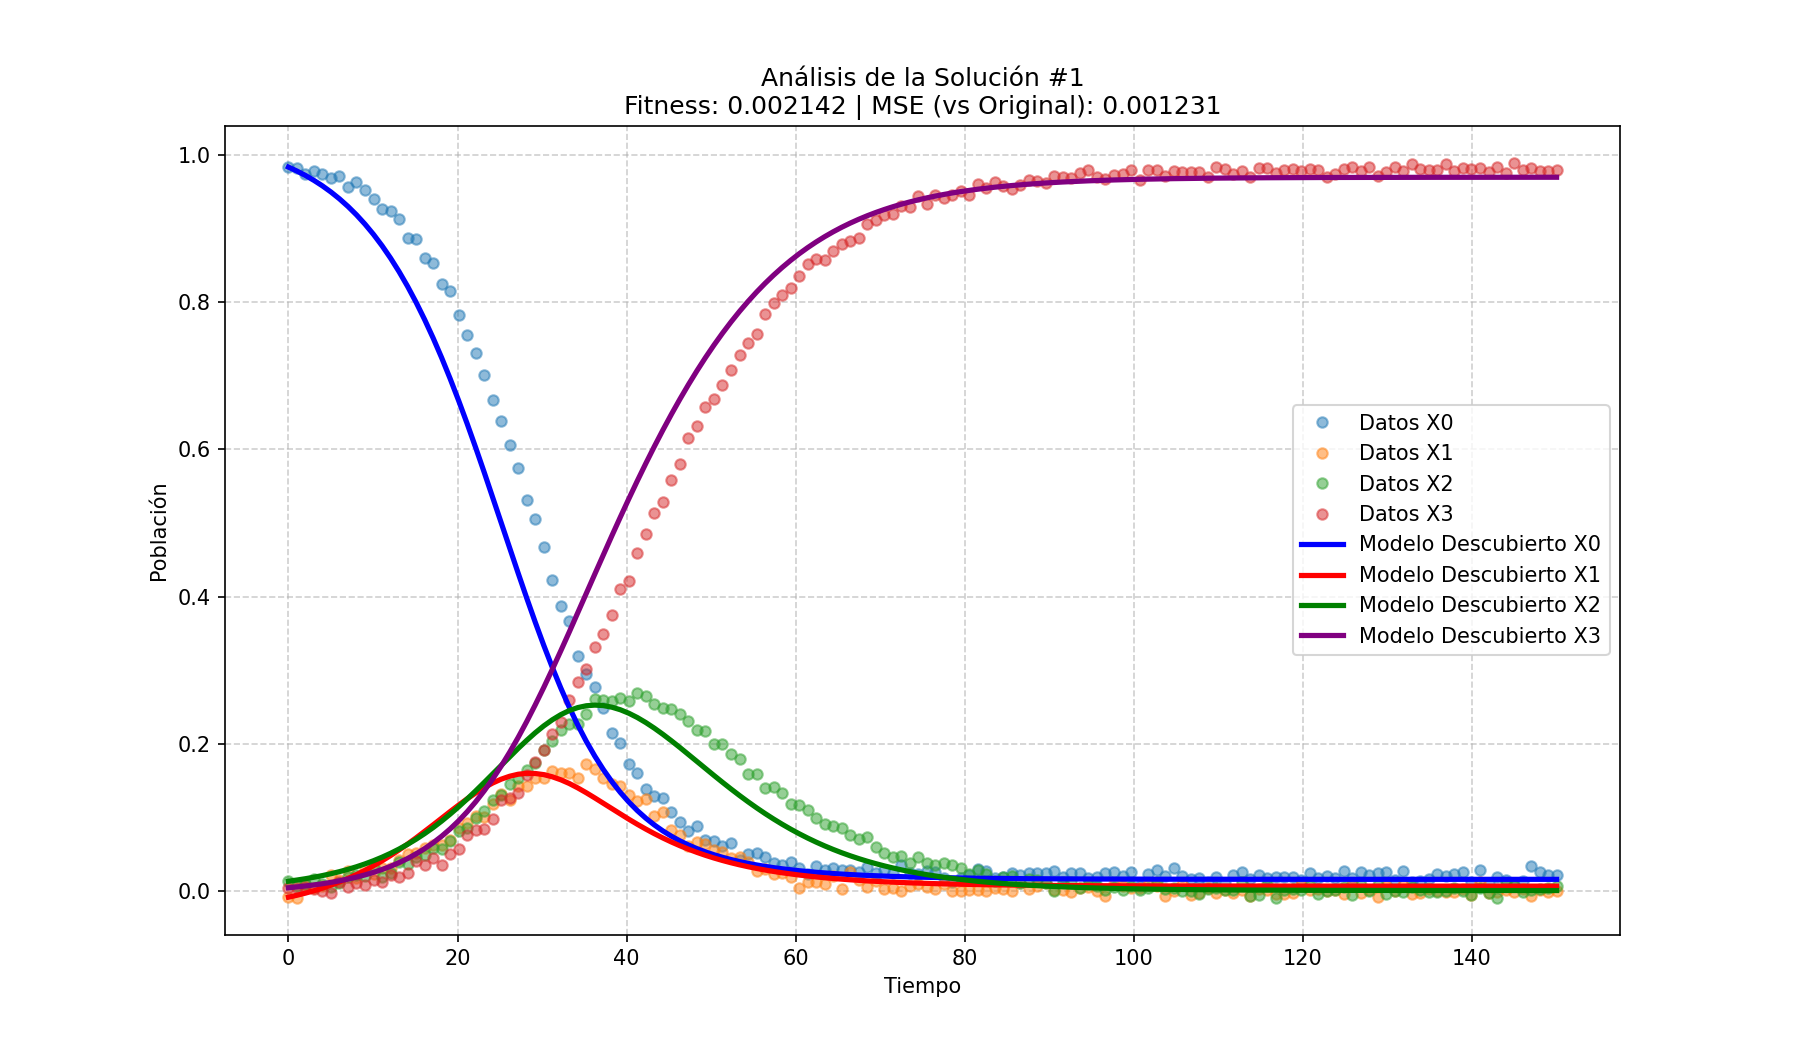
\includegraphics[width=0.7\textwidth]{Graphics/SEIR_noise_0p005_1.0_exp19__solution_1.png}
\caption{Simulación del modelo vs datos reales para 5\% de ruido, \textit{threshold} 1.0. $X_0=S$, $X_1=E$, $X_2=I$, $X_3=R$}
\label{fig:seir_5p_th10}
\end{figure}

En la Figura~\ref{fig:seir_5p_th10} se observa la excelente concordancia entre los datos generados y la simulación del modelo, incluso considerando el pequeño nivel de ruido.

Es interesante destacar que, si bien el sistema con menor \textit{fitness} fue seleccionado como la mejor solución por el algoritmo genético según su función de evaluación, la segunda mejor solución muestra un comportamiento ligeraemente más ajustado a los datos reales. En particular, esta segunda solución presenta un error cuadrático medio (MSE) de validación de apenas 0.001073, valor inferior al reportado por la mejor solución en términos de \textit{fitness}.

Este fenómeno refleja una importante distinción entre el valor de \textit{fitness} utilizado durante la evolución que incluye penalizaciones estructurales y el ajuste puro de los datos medido por el MSE. En este caso en particular la segunda mejor soluci\'on que esta mas ajustadas a los datos tiene una arista m\'as con respecto a la mejor soluci\'on calculada por la funci\'on fitness. 

La solución en cuestión genera el siguiente sistema de ecuaciones diferenciales:
\[
\begin{aligned}
\frac{dS}{dt} &= -0.31590\,SI - 6.93e-17\,IR, \\
\frac{dE}{dt} &= 0.19467\,SI - 0.45074\,EI - 0.01597\,IR, \\
\frac{I}{dt} &= 0.12123\,SI + 0.16135\,EI - 0.09800\,IR, \\
\frac{dR}{dt} &= -1.52e-16\,SI + 0.28939\,EI + 0.11895\,IR.
\end{aligned}
\]
Como se puede observar, aunque el modelo incluye algunos términos de orden muy pequeño, su desempeño en la simulación es altamente preciso. Esto se refleja en la Figura~\ref{fig:seir_5p_th10_sol2}, donde se comparan los datos observados con los obtenidos mediante la integración del sistema inferido.


\begin{figure}[H]
\centering
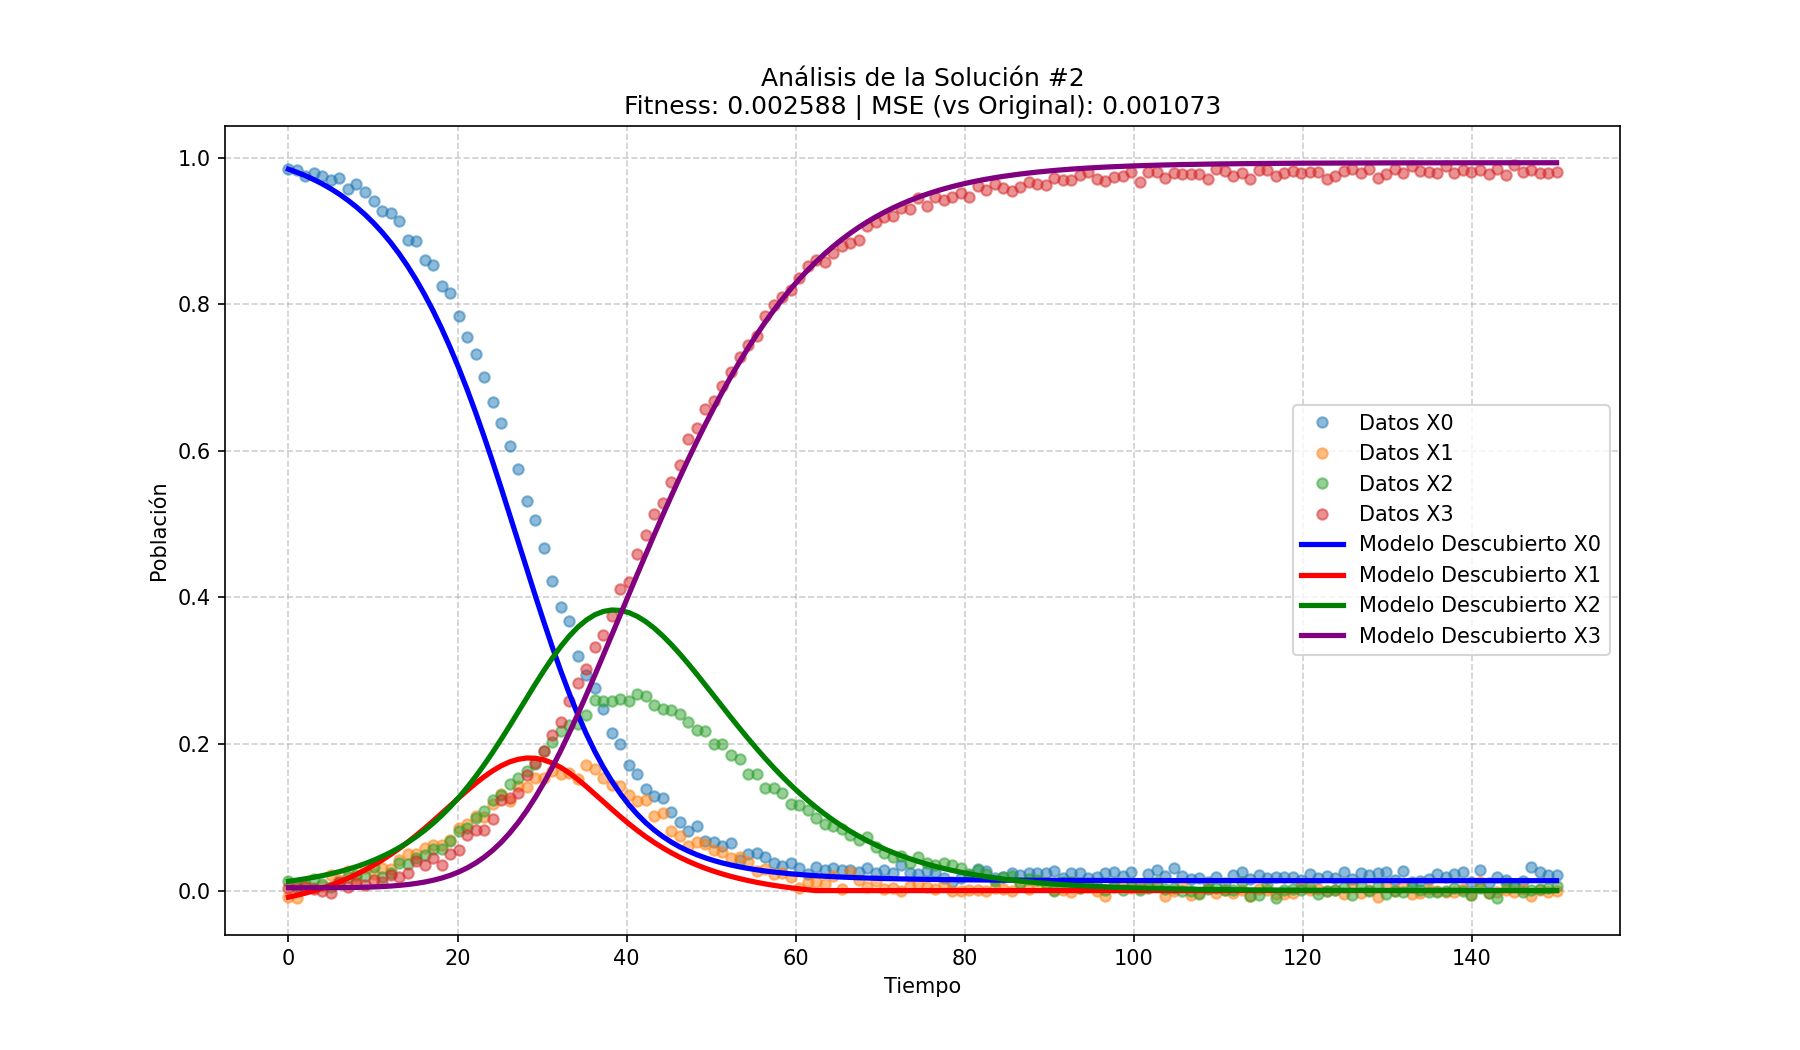
\includegraphics[width=0.7\textwidth]{Graphics/SEIR_noise_0p005_1.0_exp19__solution_2.png}
\caption{Simulación del modelo vs datos reales para 5\% de ruido, \textit{threshold} 1.0. $X_0=S$, $X_1=E$, $X_2=I$, $X_3=R$}
\label{fig:seir_5p_th10_sol2}
\end{figure}

Por otro lado, para niveles de ruido más elevados como el 30\,\%, se logran también resultados destacables. La mejor solución obtenida con \textit{threshold} de 1.0 alcanzó un error de validación de solo 0.03656, lo cual es notable dada la magnitud del ruido incorporado. El sistema inferido en este caso fue:

\[
\begin{aligned}
\frac{dS}{dt} &= -0.01150\,SI - 0.28478\,SR, \\
\frac{dE}{dt} &= 0.23812\,EI, \\
\frac{dI}{dt} &= 0.01150\,SI, \\
\frac{dR}{dt} &= 0.28478\,SR - 0.23812\,EI.
\end{aligned}
\]

\begin{figure}[H]
\centering
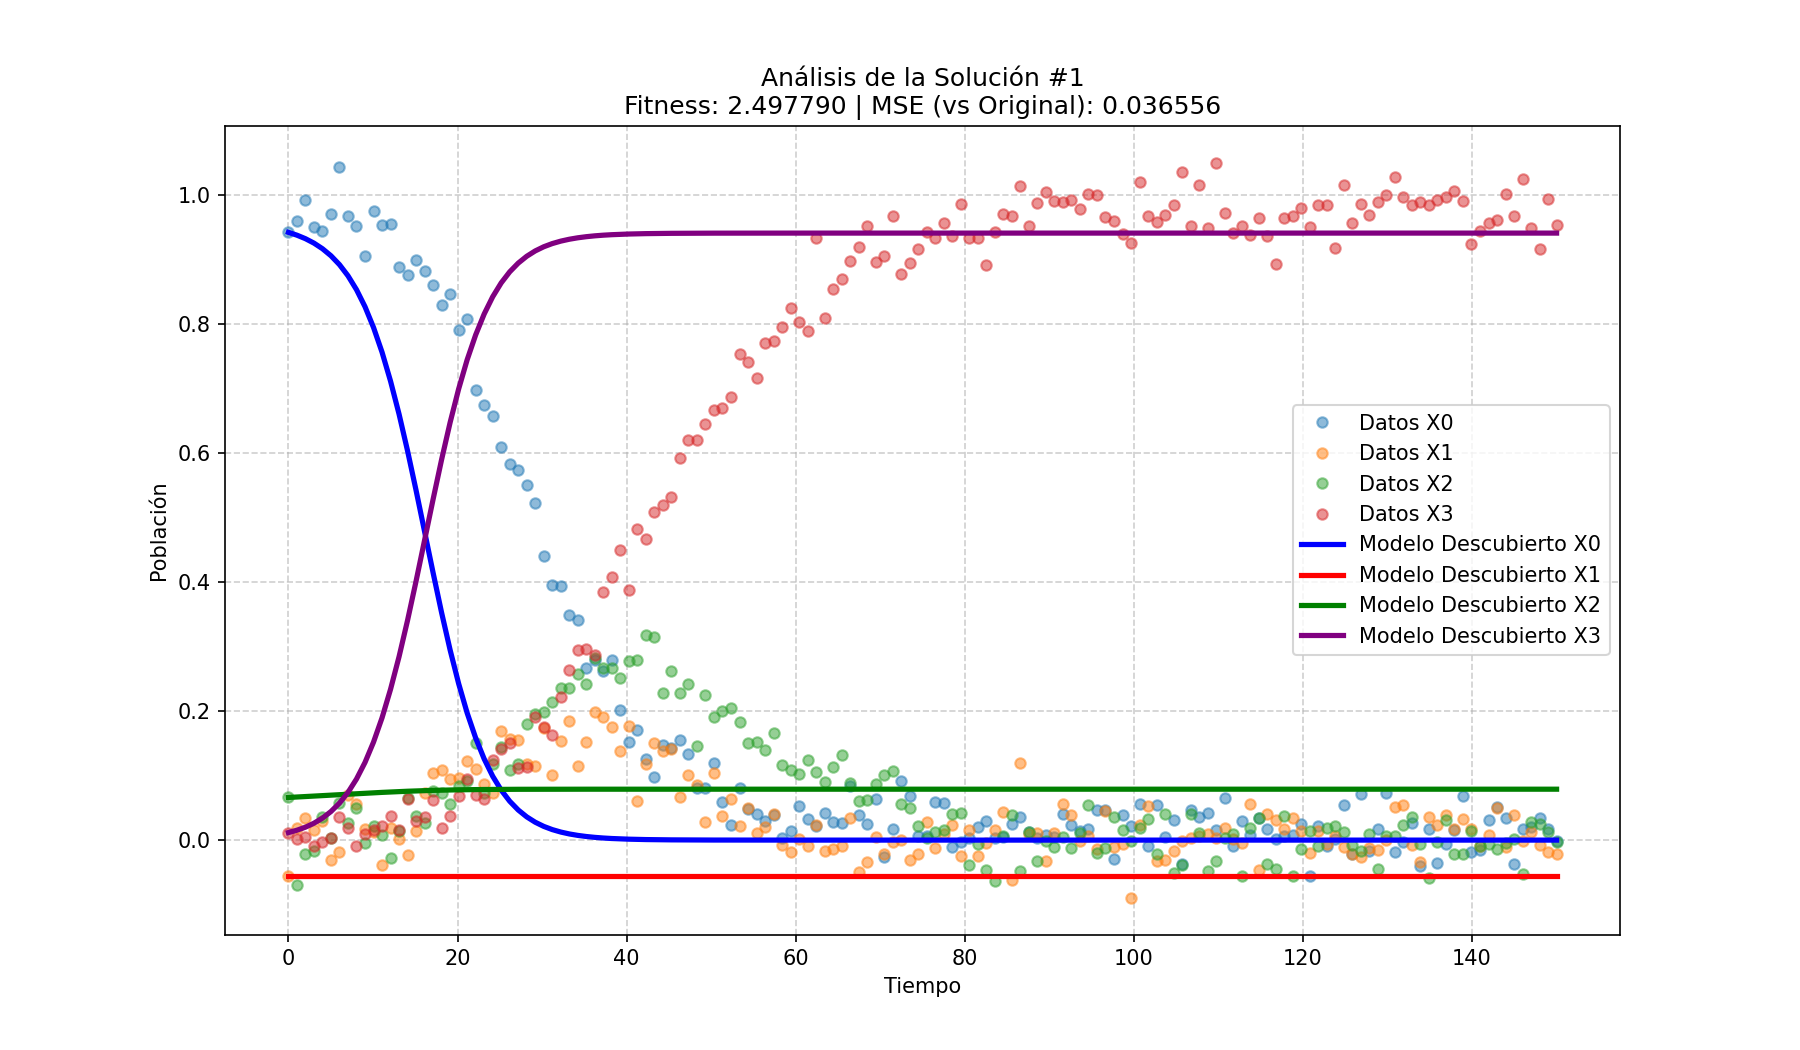
\includegraphics[width=0.7\textwidth]{Graphics/SEIR_noise_0p03_1.0_exp1__solution_1.png}
\caption{Simulación del modelo vs datos reales para 30\% de ruido, \textit{threshold} 1.0. $X_0=S$, $X_1=E$, $X_2=I$, $X_3=R$}
\label{fig:seir_30p_th10}
\end{figure}

A pesar del nivel de ruido, la forma del sistema se mantiene coherente con la estructura compartimental del modelo SEIR, recuperando de manera parcial la dinámica de transición entre compartimentos.

Es importante remarcar que, al igual que en el caso del modelo SIR, no se logró recuperar exactamente la formulación original del modelo generador. Sin embargo, las soluciones inferidas presentan estructuras de grafo razonables y dinámicamente coherentes, ajustándose correctamente a los datos generados, la mejor soluci\'on devuelta contiene todas las aristas del grafo del modelo SEIR. En escenarios con mayor ruido, el algoritmo introduce términos adicionales que probablemente compensan las oscilaciones inducidas por la perturbación estocástica. Aun así, el \textit{fitness} global y los valores de MSE validan la utilidad de las soluciones obtenidas.

Adicionalmente, los tiempos de ejecución promedio del algoritmo genético para cada configuración oscilaron entre los 4 minutos y 24 segundos hasta 5 minutos por experimento. Dependiendo del tamaño de la población, el número de generaciones y la complejidad del grafo inferido estos tiempos son aceptables, considerando la alta dimensionalidad del espacio de búsqueda inducido por todas las posibles configuraciones de grafos válidos y sistemas de ecuaciones asociados.

A continuaci\'on se muestran los resultados de los experimentos del modelo SIRD.


\subsection{Modelo SIRD}

El modelo SIRD es una extensión del clásico modelo SIR y proporciona un marco matemático para analizar la propagación de una enfermedad infecciosa que puede tener un desenlace fatal \cite{Hethcote2000}. El sistema se define mediante el siguiente conjunto de ecuaciones diferenciales:
%
\[
\begin{aligned}
    \frac{dS}{dt} &= -\frac{\beta SI}{S+I+R} , \\
    \frac{dI}{dt} &= \frac{\beta SI}{S+I+R} - \gamma I - \mu I, \\
    \frac{dR}{dt} &= \gamma I, \\
    \frac{dD}{dt} &= \mu I.
\end{aligned}
\]
%
Donde S representa la proporción de individuos susceptibles, I los infecciosos, R los recuperados (y con inmunidad), y D los fallecidos a causa de la enfermedad. El parámetro $\beta$ controla la tasa de transmisión, $\gamma$ es la tasa de recuperación, y $\mu$ representa la tasa de mortalidad del agente infeccioso.

El grafo que representa este sistema está compuesto por las siguientes aristas, que ilustran las transiciones posibles entre los compartimentos: $S \rightarrow I$, $I \rightarrow R$, y $I \rightarrow D$.

Se utilizaron como valores de los parámetros $\beta = 0.5$, $\gamma = 0.1$ y $\mu=0.2$ con punto inicial (0.7, 0.3, 0, 0) y se integró en el intervalo $0 \leq t \leq 150$ para obtener los datos que aparecen en la imagen~\ref{fig:sird_sin_ruido}. Del conjunto de puntos se seleccionaron 150 muestras como datos para el algoritmo gen\'etico. 

\begin{figure}[H]
\centering
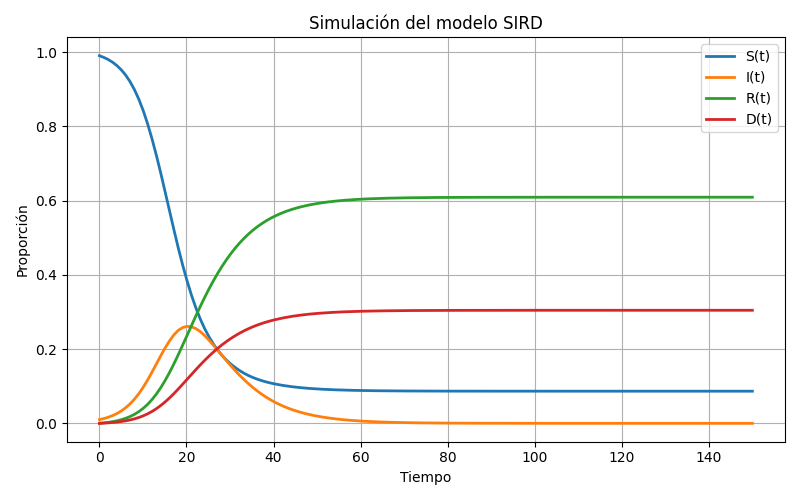
\includegraphics[width=0.7\textwidth]{Graphics/sird_sin_ruido.png}
\caption{Datos simulados del modelo SIRD}
\label{fig:sird_sin_ruido}
\end{figure}

El algoritmo genético fue aplicado usando una población inicial de 30 individuos y 20 generaciones, considerando distintas configuraciones de ruido \( 5\%, 15\%, 30\% \) y valores de \textit{threshold} (0.8 y 1.0). Los resultados obtenidos se resumen en la Tabla~\ref{tab:resumen-sird}.

\begin{table}[H]
\centering
\caption{Resultados experimentales del modelo SIRD bajo diferentes configuraciones}
\label{tab:resumen-sird}
\begin{tabular}{|c|c|c|c|c|}
\hline
\textbf{Ruido} & \textbf{Threshold} & \textbf{MSE Validación} & \textbf{Fitness} & \textbf{Aristas del Grafo} \\
\hline
5\% & 0.8 & 0.171315 & 0.189132 & 0$\rightarrow$2, 1$\rightarrow$2, 2$\rightarrow$1, 3$\rightarrow$2\\
5\% & 1.0 & 0.193155 & 0.210042 & 0$\rightarrow$2, 1$\rightarrow$2, 2$\rightarrow$1, 2$\rightarrow$3\\
15\% & 0.8 & 0.327456 & 0.372651 & 0$\rightarrow$2, 0$\rightarrow$3, 1$\rightarrow$3\\
15\% & 1.0 & 0.060112 & 0.024381 & 0$\rightarrow$1, 1$\rightarrow$2, 2$\rightarrow$3\\
30\% & 0.8 & 0.322215 & 2.323537 & 0$\rightarrow$1, 0$\rightarrow$2, 0$\rightarrow$3\\
30\% & 1.0 & 0.322215 & 2.323537 & 0$\rightarrow$2, 1$\rightarrow$2, 2$\rightarrow$3\\
\hline
\end{tabular}
\end{table}

% Se observa que configuraciones con menor nivel de ruido (5\%) generan resultados consistentes con errores relativamente bajos. En particular, con ruido del 5\% y \textit{threshold} de 0.8 se obtuvo el mejor desempeño relativo a las otras configuraciones con el mismo nivel de ruido. Al aumentar el ruido hasta el 15\%, la configuración con \textit{threshold} de 1.0 mostró un desempeño significativamente mejor en términos de fitness (0.024381) y MSE (0.060112) respecto al caso con \textit{threshold} de 0.8.

A continuación se detallan las ecuaciones diferenciales correspondientes a una de las mejores soluciones obtenidas en los experimentos, específicamente con un nivel de ruido del 15\% y un \textit{threshold} de 1.0. Esta configuración destacó notablemente por lograr un ajuste preciso a los datos experimentales (de manera consistente en los 30 experimentos), reflejado en un bajo valor de MSE (0.060112) y excelente valor de \textit{fitness} (0.024381). El sistema inferido en este caso es:

\[
\begin{aligned}
\frac{dS}{dt} &= -0.34662\,S I, \\
\frac{dI}{dt} &= 0.34662\,S I - 0.23721\,I R, \\
\frac{dR}{dt} &= -0.24310\,S D + 0.23721\,I R - 1.19084\,I D - 1.83079\,R D - 2.97057\,D^2 - 0.85770\,D, \\
\frac{dD}{dt} &= 0.24310\,S D + 1.19084\,I D + 1.83079\,R D + 2.97057\,D^2 + 0.85770\,D.
\end{aligned}
\]

\begin{figure}[H]
\centering
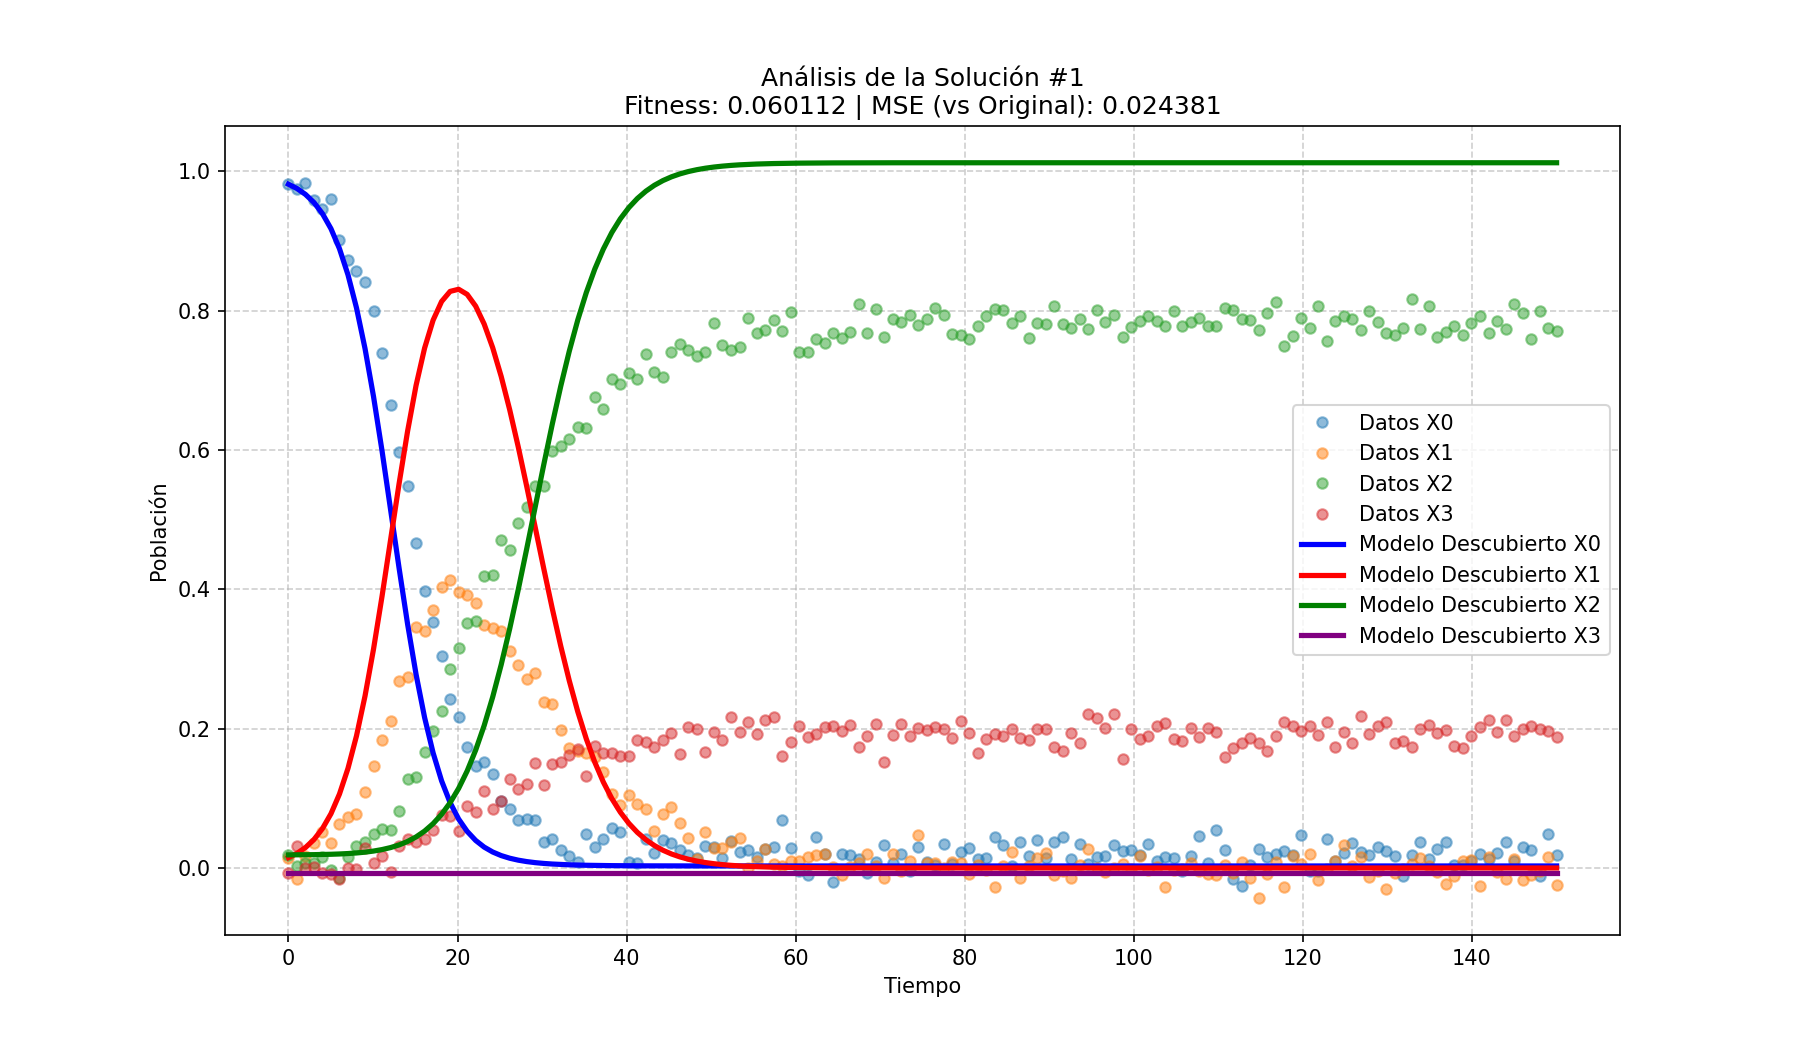
\includegraphics[width=0.7\textwidth]{Graphics/SIRD_noise_0p015_1.0_exp1__solution_1.png}
\caption{Simulación del modelo vs datos reales para 15\% de ruido, \textit{threshold} 1.0. $X_0=S$, $X_1=I$, $X_2=R$, $X_3=D$}
\label{fig:sird_15p_th10}
\end{figure}

Estos resultados muestran cómo, pese al ruido considerable presente en los datos, el algoritmo logró identificar correctamente relaciones significativas entre los compartimentos del modelo SIRD. Se observa, sin embargo, la introducción de términos adicionales respecto al modelo original, que indican mecanismos compensatorios del modelo frente a la perturbación del ruido. Se puede observar en la Figura~\ref{fig:sird_15p_th10} la cercania entre los datos generados y la soluci\'on encontrada.

Sin embargo, las soluciones halladas con otras configuraciones de par\'ametros (ruido y threshold), no se ajustan muy bien a los datos, y al alcanzar niveles altos de ruido (30\%), el desempeño del modelo inferido decae sustancialmente, reflejado en un incremento significativo del valor del fitness y del MSE, indicando dificultad para capturar las dinámicas originales del modelo SIRD con alta perturbación en los datos.

Se presenta el segundo conjunto de soluciones que mejor se ajustan a los datos, correspondientes al escenario con un 5\% de ruido y \textit{threshold} de 0.8. Aunque esta solución obtuvo valores considerablemente superiores en términos de error cuadrático medio (MSE de 0.171315) y \textit{fitness} (0.189132), sigue siendo relevante para entender la variabilidad de los resultados inferidos respecto al nivel de ruido. Las ecuaciones diferenciales inferidas en este caso son:

$$
\begin{aligned}
\frac{dS}{dt} &= -0.29877\,S I - 0.02877\,I R - 0.04429\,R^2 - 0.18030\,R D, \\
\frac{dI}{dt} &= 4.73 \times 10^{-15}\,I R - 8.33 \times 10^{-17}ID\, - 7.69 \times 10^{-15}\,R^2\, - 1.71 \times 10^{-15} R D, \\
\frac{dR}{dt} &= 0.29877\,S I + 0.02877\,I R + 0.73276\,I D + 0.04429\,R^2 + 0.18030\,R D + 3.69095\,D^2 + 0.72146\,D, \\
\frac{dD}{dt} &= -0.73276\,I D - 3.69095\,D^2 - 0.72146\,D.
\end{aligned}
$$

\begin{figure}[H]
\centering
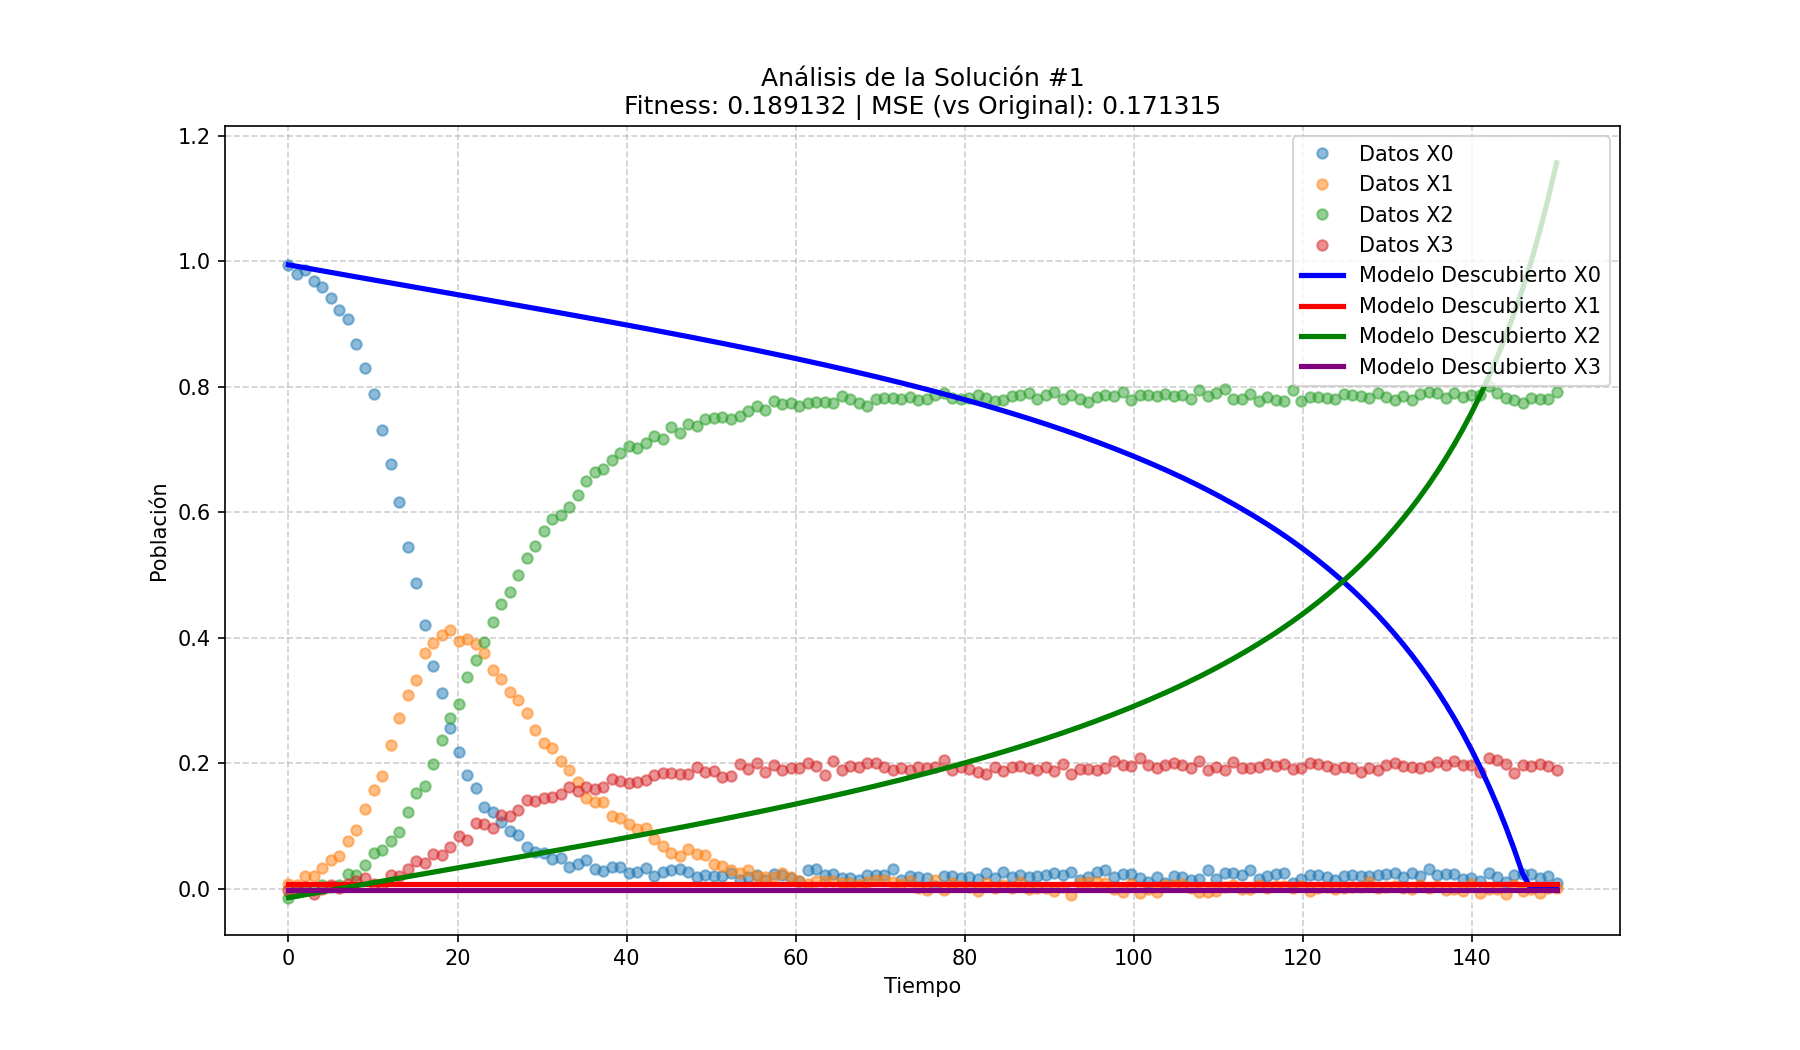
\includegraphics[width=0.7\textwidth]{Graphics/SIRD_noise_0p005_0.8_exp1__solution_1.png}
\caption{Simulación del modelo vs datos reales para 15\% de ruido, \textit{threshold} 1.0. $X_0=S$, $X_1=I$, $X_2=R$, $X_3=D$}
\label{fig:sird_5p_th08}
\end{figure}

La Figura~\ref{fig:sird_5p_th08} muestra gráficamente la simulación del modelo inferido en comparación con los datos originales generados bajo estas condiciones experimentales.

En esta figura se observa claramente que, aunque el modelo capturó parcialmente las tendencias generales, presenta mayores desviaciones respecto a los datos originales en comparación con la mejor solución previamente analizada. Esto subraya la importancia crítica del nivel de ruido y el \textit{threshold} elegido para obtener modelos más precisos y robustos.

En términos de rendimiento computacional, el tiempo requerido para cada ejecución del algoritmo genético se mantuvo en un rango de 3 minutos y 48 segundos a 4 minutos y 53 segundos. Este rendimiento se considera razonable dada la carga computacional que imponen un sistema con cuatro compartimentos.

En la proxima secci\'on se exponen los resultados de la experimentaci\'on con el modelo SEIRV.

\subsection{Modelo SEIRV}

El modelo SEIRV amplía el marco del modelo SEIR para incluir el efecto de las campañas de vacunación en la dinámica de una enfermedad. Este enfoque proporciona una herramienta matemática para evaluar cómo la inmunización interviene en la propagación de una infección que posee un período de latencia \cite{Anderson1991}. El sistema se define mediante el siguiente conjunto de ecuaciones diferenciales:

\[
\begin{aligned}
    \frac{dS}{dt} &= -\frac{\beta SI}{N} - \nu S, \\
    \frac{dE}{dt} &= \frac{\beta SI}{N} - \alpha E, \\
    \frac{dI}{dt} &= \alpha E - \gamma I, \\
    \frac{dR}{dt} &= \gamma I, \\
    \frac{dV}{dt} &= \nu S.
\end{aligned}
\]

Donde $N = S+E+I+R+V$. Las variables representan la proporción de individuos: \textbf{S} (susceptibles), \textbf{E} (expuestos, en período de incubación), \textbf{I} (infecciosos), \textbf{R} (recuperados) y \textbf{V} (vacunados). Los parámetros del modelo son: $\beta$ para la tasa de transmisión, $\alpha$ la tasa de progresión de expuesto a infeccioso, $\gamma$ la tasa de recuperación, y $\nu$ la tasa de vacunación sobre la población susceptible.

El grafo que representa este sistema está compuesto por las siguientes aristas, que ilustran las transiciones posibles: $S \rightarrow E$, $S \rightarrow V$, $E \rightarrow I$ y $I \rightarrow R$.

Se utilizaron como valores de los parámetros $\beta = 0.5$, $\alpha = 0.2$, $\gamma = 0.1$ y $\nu = 0.05$ con punto inicial (0.9, 0.1, 0, 0, 0) y se integró en el intervalo $0 \leq t \leq 150$ para obtener los datos que aparecen en la Figura~\ref{fig:seirv_sin_ruido}. Del conjunto de puntos se seleccionaron 150 muestras como datos para el algoritmo genético.

\begin{figure}[H]
    \centering
    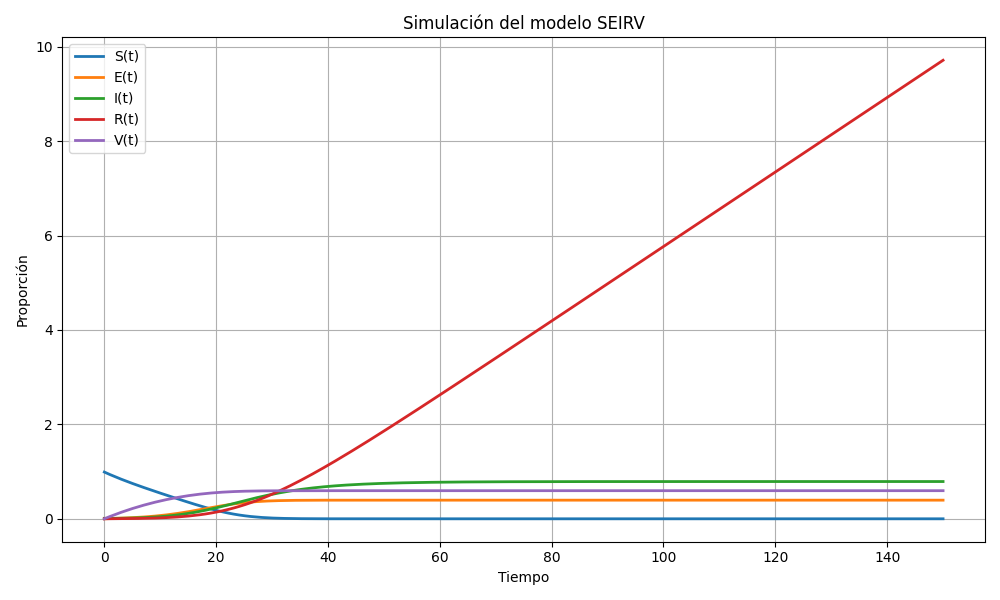
\includegraphics[width=0.7\textwidth]{Graphics/seirv_sin_ruido.png}
    \caption{Datos simulados del modelo SEIRV}
    \label{fig:seirv_sin_ruido}
\end{figure}

El algoritmo genético fue aplicado usando una población inicial de 40 individuos y 40 generaciones, considerando distintas configuraciones de ruido \( 5\%, 15\%, 30\% \) y valores de \textit{threshold} (0.8 y 1.0).Los resultados obtenidos se resumen en la Tabla~\ref{tab:resumen-seirv}.

\begin{table}[H]
\centering
\caption{Resultados experimentales del modelo SEIRV bajo diferentes configuraciones}
\label{tab:resumen-seirv}
\begin{tabular}{|c|c|c|c|c|}
\hline
\textbf{Ruido} & \textbf{Threshold} & \textbf{MSE Validación} & \textbf{Fitness} & \textbf{Aristas del Grafo} \\
\hline
5\% & 0.8 & 3.29928170 & 3.61697174 & 0$\rightarrow$3, 1$\rightarrow$3, 1$\rightarrow$4, 2$\rightarrow$1, 2$\rightarrow$3, 4$\rightarrow$2\\
5\% & 1.0 & 3.70048194 & 3.84277075 & 0$\rightarrow$3, 1$\rightarrow$3, 2$\rightarrow$1, 4$\rightarrow$1, 4$\rightarrow$3\\
15\% & 0.8 & 3.58154992 & 4.08872264 & 0$\rightarrow$2, 0$\rightarrow$4, 2$\rightarrow$3, 4$\rightarrow$1, 4$\rightarrow$2\\
15\% & 1.0 & 3.45445046 & 4.09157519 & 0$\rightarrow$1, 0$\rightarrow$4, 2$\rightarrow$0, 2$\rightarrow$3, 3$\rightarrow$1, 4$\rightarrow$2\\
30\% & 0.8 & 3.97527256 & 4.31880023 & 0$\rightarrow$4, 1$\rightarrow$2, 3$\rightarrow$1, 4$\rightarrow$3\\
30\% & 1.0 & 4.09472754 & 4.47803501 & 0$\rightarrow$1, 0$\rightarrow$3, 1$\rightarrow$2, 1$\rightarrow$3, 2$\rightarrow$4\\
\hline
\end{tabular}
\end{table}

A diferencia de los modelos anteriores, la inferencia del modelo SEIRV presentó una mayor complejidad, reflejada en valores de MSE y \textit{fitness} considerablemente más altos en todas las configuraciones. A continuación, se analizan las mejores soluciones obtenidas para cada nivel de ruido.

Para un nivel de ruido del 5\%, la mejor solución se encontró con un \textit{threshold} de 0.8, obteniendo un MSE de validación de 3.299. El sistema de ecuaciones inferido es el siguiente:
\[
\begin{aligned}
\frac{dS}{dt} &= -0.25372\,S V, \\
\frac{dE}{dt} &= -0.33050\,S E - 0.02951\,S V - 0.79277\,E^2 - 0.63327\,E I + 0.51342\,E, \\
\frac{dI}{dt} &= -3.75503\,S E - 1.80538\,S I - 4.61293\,E^2 - 1.96860\,E I + 2.42742\,E V \\ & \quad - 3.13577\,E - 0.90574\,I V - 1.48401\,I, \\
\frac{dR}{dt} &= 3.70352\,S E + 1.80538\,S I + 0.25372\,S V + 4.24854\,E^2 + 2.58864\,E I \\ & \quad + 1.67204\,E + 0.90574\,I V + 1.48401\,I, \\
\frac{dV}{dt} &= 0.38201\,S E + 0.02951\,S V + 1.15716\,E^2 + 0.01324\,E I - 2.42742\,E V + 0.95030\,E.
\end{aligned}
\]
\begin{figure}[H]
    \centering
    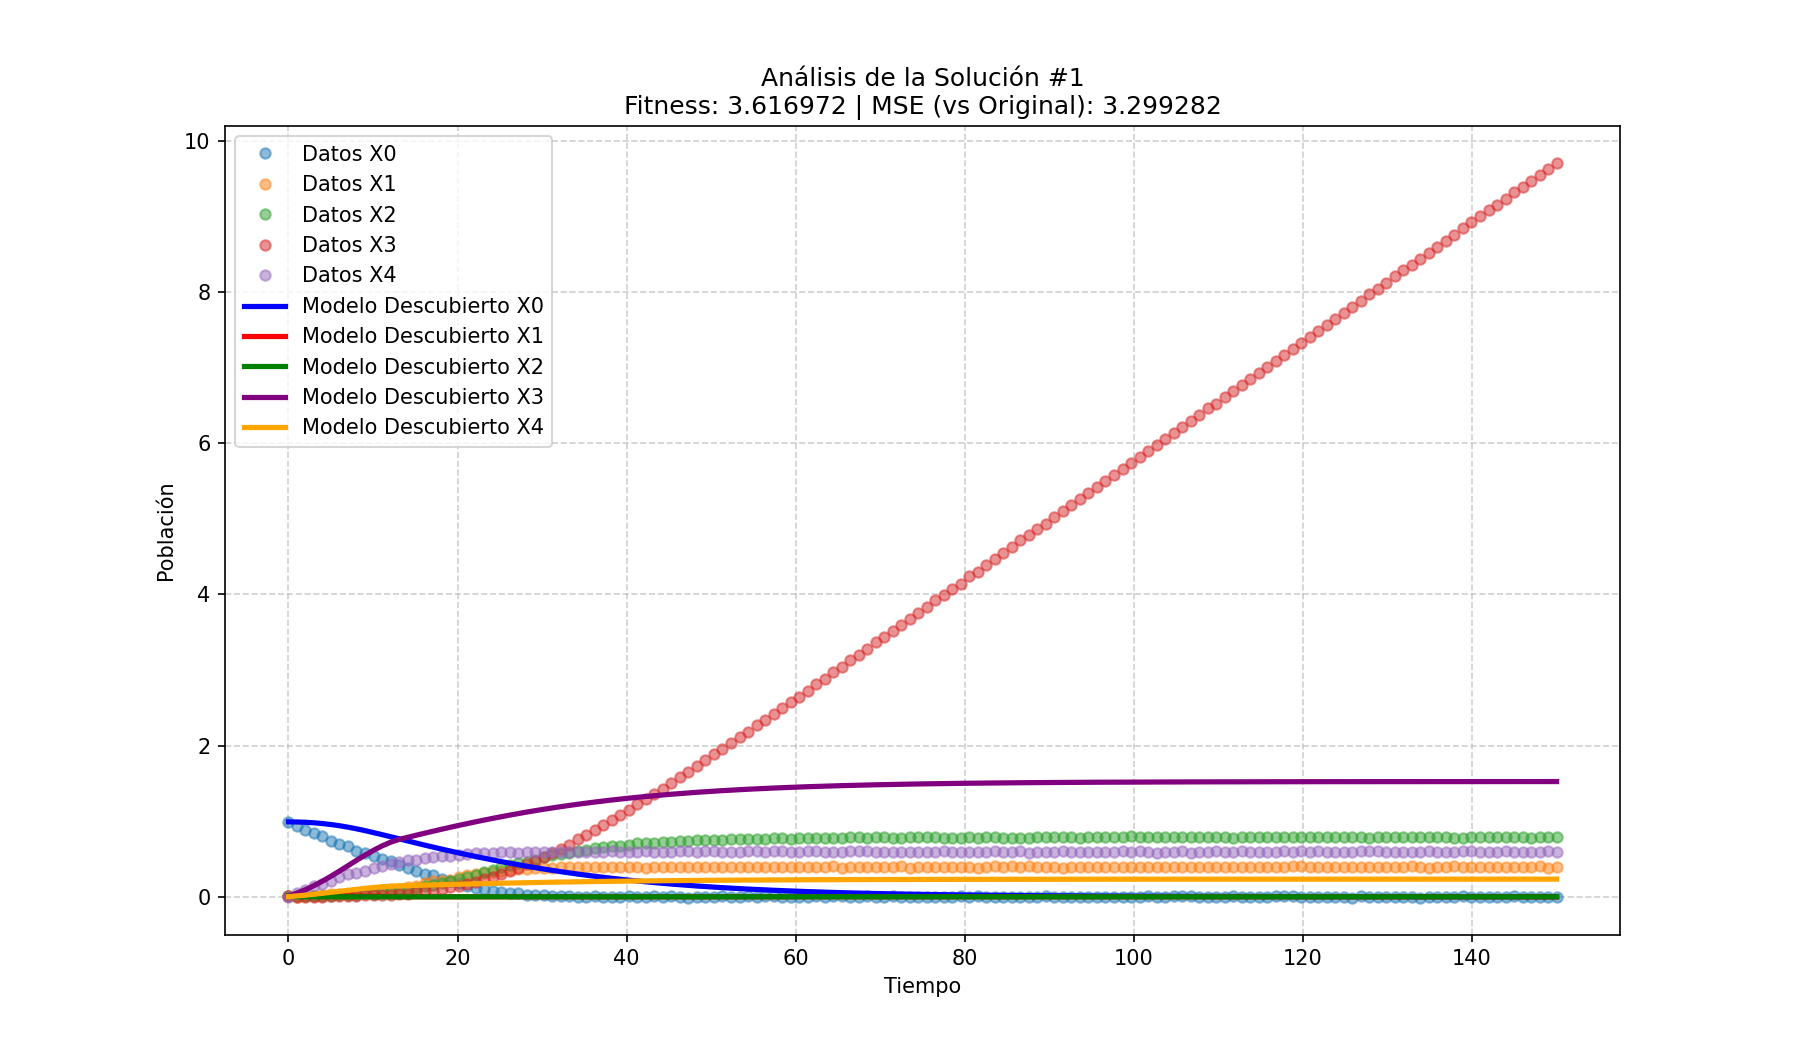
\includegraphics[width=0.7\textwidth]{Graphics/SEIRV_noise_0p005_0.8_exp2__solution_1.png}
    \caption{Simulación del mejor modelo SEIRV vs datos reales para 5\% de ruido, \textit{threshold} 0.8. ($X_0=S, X_1=E, X_2=I, X_3=R, X_4=V$)}
    \label{fig:seirv_5p_th08}
\end{figure}

Al incrementar el ruido al 15\%, el mejor resultado se obtuvo con un \textit{threshold} de 1.0, alcanzando un MSE de validación de 3.454. Este valor, aunque elevado, fue el más bajo para este nivel de ruido. Las ecuaciones inferidas fueron:
\[
\begin{aligned}
\frac{dS}{dt} &= -0.72788\,S E + 0.25454\,S V - 0.03815\,S - 0.78280\,E V - 0.04831\,V^2 - 0.22807\,V, \\
\frac{dE}{dt} &= 0.57364\,S E + 0.03439\,S V + 0.14612\,E V, \\
\frac{dI}{dt} &= -0.13629\,S E - 0.28893\,S V - 0.15875\,E I + 0.57387\,E V + 0.35234\,V^2 + 0.30526\,V, \\
\frac{dR}{dt} &= -0.19364\,S E + 0.23142\,E I - 0.03907\,E V, \\
\frac{dV}{dt} &= 0.48417\,S E + 0.03815\,S - 0.07267\,E I + 0.10188\,E V - 0.30403\,V^2 - 0.07718\,V.
\end{aligned}
\]
\begin{figure}[H]
    \centering
    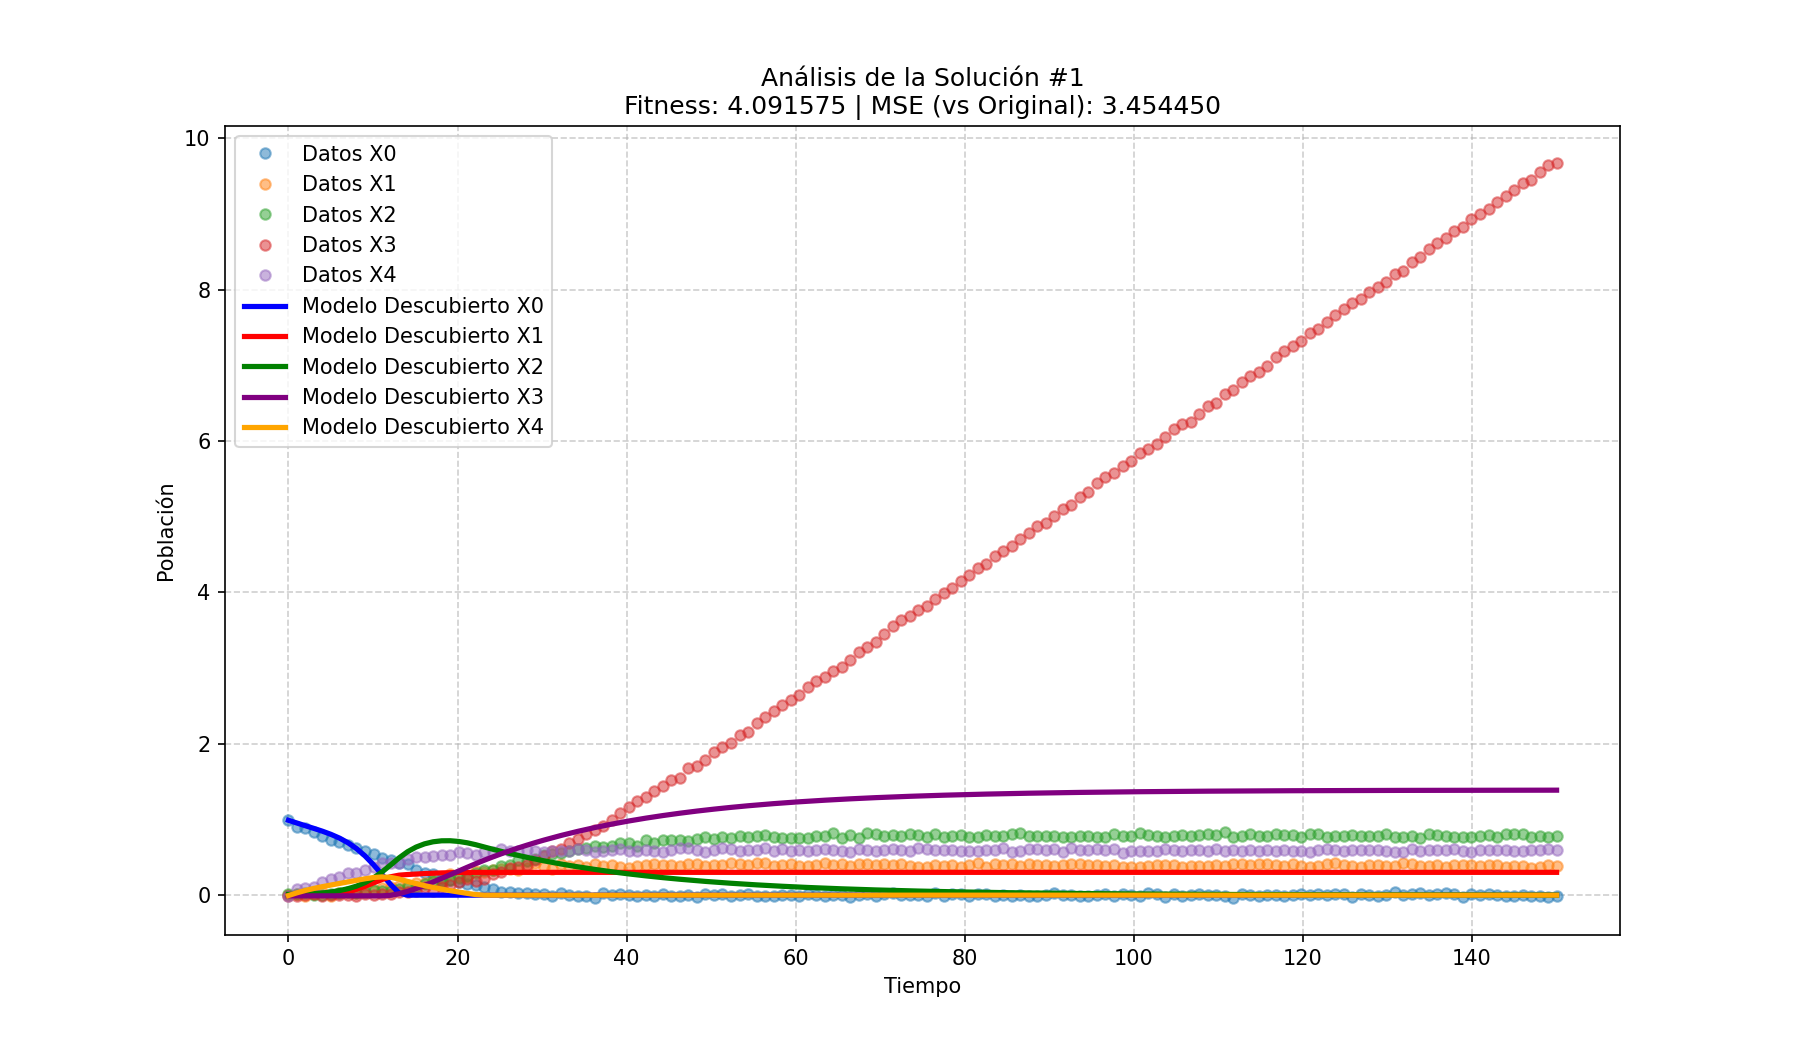
\includegraphics[width=0.7\textwidth]{Graphics/SEIRV_noise_0p015_1.0_exp1__solution_1.png}
    \caption{Simulación del mejor modelo SEIRV vs datos reales para 15\% de ruido, \textit{threshold} 1.0. ($X_0=S, X_1=E, X_2=I, X_3=R, X_4=V$)}
    \label{fig:seirv_15p_th10}
\end{figure}

Finalmente, con un 30\% de ruido, la solución con menor error (MSE de 3.975) volvió a corresponder a un \textit{threshold} de 0.8. El sistema resultante, aunque muy alejado del modelo teórico, representa el mejor ajuste encontrado bajo estas condiciones de alta incertidumbre.
\[
\begin{aligned}
\frac{dS}{dt} &= -0.66931\,S I, \\
\frac{dE}{dt} &= -0.41171\,S E - 0.40749\,S I + 0.20785\,E V + 0.17254\,E, \\
\frac{dI}{dt} &= 0.69568\,S E + 0.40749\,S I + 0.03826\,E, \\
\frac{dR}{dt} &= -0.28397\,S E - 0.16943\,E V - 0.21079\,E + 0.06849\,I V, \\
\frac{dV}{dt} &= 0.66931\,S I - 0.03842\,E V - 0.06849\,I V.
\end{aligned}
\]
\begin{figure}[H]
    \centering
    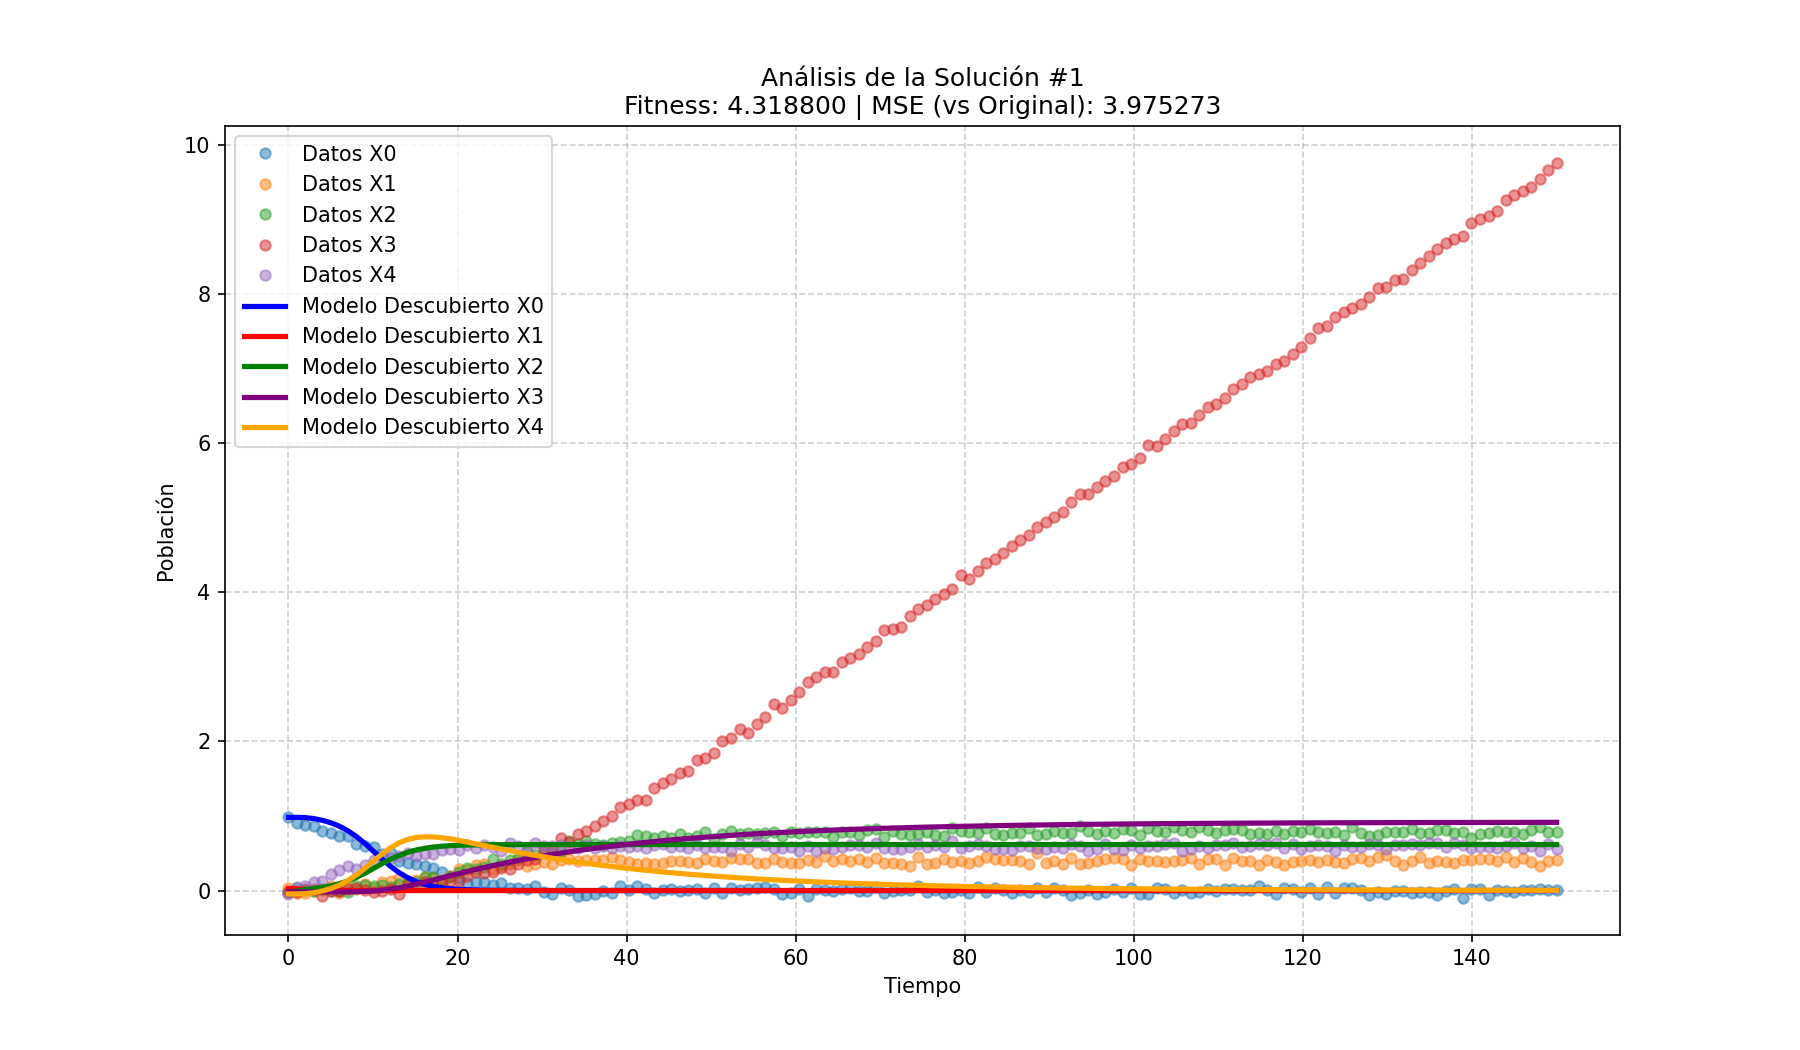
\includegraphics[width=0.7\textwidth]{Graphics/SEIRV_noise_0p03_0.8_exp1__solution_1.png}
    \caption{Simulación del mejor modelo SEIRV vs datos reales para 30\% de ruido, \textit{threshold} 0.8. ($X_0=S, X_1=E, X_2=I, X_3=R, X_4=V$)}
    \label{fig:seirv_30p_th08}
\end{figure}

Adicionalmente, es relevante mencionar los tiempos de ejecución para los experimentos del modelo SEIRV. Dada la mayor complejidad del sistema, con cinco compartimentos, y el aumento en los parámetros del algoritmo genético (40 individuos y 40 generaciones), los tiempos por experimento oscilaron entre 8 minutos y 57 segundos y 10 minutos con 12 segundos.

En resumen, los experimentos con el modelo SEIRV demuestran las limitaciones del método frente a sistemas de mayor dimensionalidad y complejidad. Los valores de MSE obtenidos son significativamente más altos que en los modelos previos, y las estructuras de los grafos y ecuaciones inferidas divergen considerablemente del modelo teórico. Es crucial destacar que los resultados sugieren que no existe una receta exacta o una configuración de parámetros (como el \textit{threshold}) que garantice el mejor resultado de manera consistente. En los casos analizados, las mejores soluciones se alternaron entre un \textit{threshold} de 0.8 y 1.0, lo que indica que la elección óptima de este parámetro depende intrínsecamente del nivel de ruido y de las características específicas de los datos, requiriendo un proceso de ajuste y validación para cada problema particular.

En la siguiente sección se realiza un análisis de los resultados de todos
los experimentos realizados.

\section{An\'alisis de resultados}
\label{sec:experimentation4}

Los experimentos realizados muestran que el algoritmo genético propuesto es capaz de inferir sistemas compartimentales que, aunque no siempre replican exactamente las ecuaciones originales, logran capturar con notable precisión la dinámica subyacente de los datos generados. La metodología basada en grafos dirigidos y ecuaciones polinómicas cuadráticas ajustadas por mínimos cuadrados permite una exploración eficiente del espacio de modelos compartimentales posibles.

En los casos correspondientes a los modelos SIR y SEIR, los resultados obtenidos destacan por su alto grado de fidelidad en la aproximación de las trayectorias observadas, especialmente en escenarios de bajo ruido (5\%). Incluso en estos casos, si bien la estructura original del modelo no fue completamente recuperada en todos los experimentos, las ecuaciones encontradas presentan formas compatibles con la dinámica esperada, y el grafo inferido recupera correctamente las transiciones clave entre compartimentos. Además, los valores del error cuadrático medio (MSE) y del \textit{fitness} alcanzan órdenes de magnitud muy bajos, particularmente en los experimentos con \textit{threshold} 1.0 y niveles de ruido bajos, donde el sistema SEIR obtuvo un MSE tan pequeño como 0.001073.

Cabe resaltar un fenómeno interesante identificado en el modelo SEIR: la solución con menor MSE no fue la seleccionada como la mejor por el algoritmo genético, debido a que el \textit{fitness} penaliza también la complejidad estructural del sistema ,por ejemplo, el número de aristas en el grafo. La segunda mejor solución en términos de \textit{fitness} generó un sistema con una arista adicional, pero ajustó mejor los datos simulados. Este caso pone de manifiesto que la métrica de ajuste (MSE) y la función de evaluación evolutiva (\textit{fitness}) no siempre convergen en la misma solución, lo cual puede ser relevante en aplicaciones donde se prioriza la precisión sobre la simplicidad.

En el modelo SIRD, que introduce términos no lineales con fracciones en su formulación original, los resultados muestran mayor dispersión. Aunque algunas configuraciones experimentales lograron ajustes razonables, por ejemplo, MSE de 0.060112 en el caso con 15\% de ruido y \textit{threshold} 1.0, se observa una mayor presencia de términos adicionales en las ecuaciones generadas, que no están presentes en el modelo base. Esto se debe, en parte, a que el sistema inferido se basa únicamente en combinaciones polinómicas de segundo orden, mientras que el modelo real contiene divisores dependientes del total de la población. A pesar de esta limitación, el grafo inferido tiende a capturar correctamente las relaciones funcionales esenciales, aunque los coeficientes asociados tienden a desviarse o compensarse mediante términos adicionales en las ecuaciones de los compartimentos.

El modelo SEIRV constituye el caso más complejo evaluado. Los resultados obtenidos para este modelo presentan mayores dificultades en la aproximación de las trayectorias originales, especialmente en presencia de ruido. Esto se debe a que la formulación original del modelo incluye un término fraccional dependiente del total poblacional \( N \), lo cual no puede ser directamente representado por el espacio funcional polinómico restringido a combinaciones cuadráticas de las variables. Las soluciones encontradas intentan aproximar esta dinámica utilizando combinaciones aditivas o cuadráticas de compartimentos, pero esto introduce errores sistemáticos en la simulación del comportamiento poblacional. Adicionalmente, el aumento en la dimensionalidad del sistema (cinco compartimentos) incrementa significativamente el espacio de búsqueda y complejiza la evaluación del grafo, afectando negativamente el rendimiento del algoritmo.

En general, se observa que para sistemas con bajo número de compartimentos (como SIR o SEIR), el algoritmo logra una convergencia eficiente hacia soluciones bien ajustadas, incluso en presencia de ruido. A medida que se incrementa el tamaño del sistema y la complejidad funcional ,por ejemplo, en SEIRV o modelos con divisores como SIRD, la calidad del ajuste tiende a deteriorarse, y los sistemas inferidos incorporan términos adicionales para intentar compensar los efectos del ruido o de la no linealidad estructural no modelable directamente. 

Aunque cabe mencionar que estos modelos complejos que no se ajustaron bien a los datos se ejecutaron con un numero bajo de par\'ametros para el algoritmo gen\'etico si tenemos en cuenta el espacio de busqueda, ya que una poblaci\'on inicial de 30 o 40 individuos no es una cantidad representativa.

En todos los experimentos se evidenció una relación clara entre el nivel de ruido y el desempeño del algoritmo: a menor ruido, se obtienen modelos más simples, con menos aristas en el grafo, y mejores valores de MSE. A mayor ruido, las soluciones tienden a complejizarse, incluyendo términos no presentes en el modelo original, con el objetivo de mitigar el impacto de la variabilidad estocástica. Esta tendencia se acentúa cuando se emplean umbrales de \textit{threshold} más bajos, lo que permite la inclusión de términos marginales con bajo peso.

Finalmente, los tiempos de ejecución se mantuvieron dentro de márgenes razonables: entre 40 segundos y 9 minutos por ejecución, dependiendo del modelo evaluado, el tamaño poblacional y el número de generaciones. Considerando el tamaño del espacio de búsqueda (número de grafos dirigidos válidos) y la necesidad de integración numérica para cada individuo en cada generación, estos tiempos son aceptables y reflejan la eficiencia computacional del enfoque implementado.

En resumen, el algoritmo propuesto demuestra ser efectivo para la inferencia de modelos compartimentales bajo restricciones estructurales y polinómicas. Su desempeño es sobresaliente en modelos de baja complejidad y robusto ante ruido moderado. En modelos más complejos o con formulaciones no polinómicas (como divisores dependientes de variables), su capacidad de ajuste disminuye, aunque logra encontrar aproximaciones estructuralmente coherentes. El diseño de nuevas estrategias que permitan ampliar el espacio funcional de las ecuaciones generadas podría mejorar estos resultados en futuras investigaciones.


